\chapter{HASIL DAN PEMBAHASAN}

\section{Hasil Rancangan Sistem Identifikasi Kendaraan Pada Pemarkiran Dengan Pengenalan Citra Dan Pembacaan RFID}

\subsection{Hasil Perancangan Perangkat Keras}
\begin{figure} [H]
    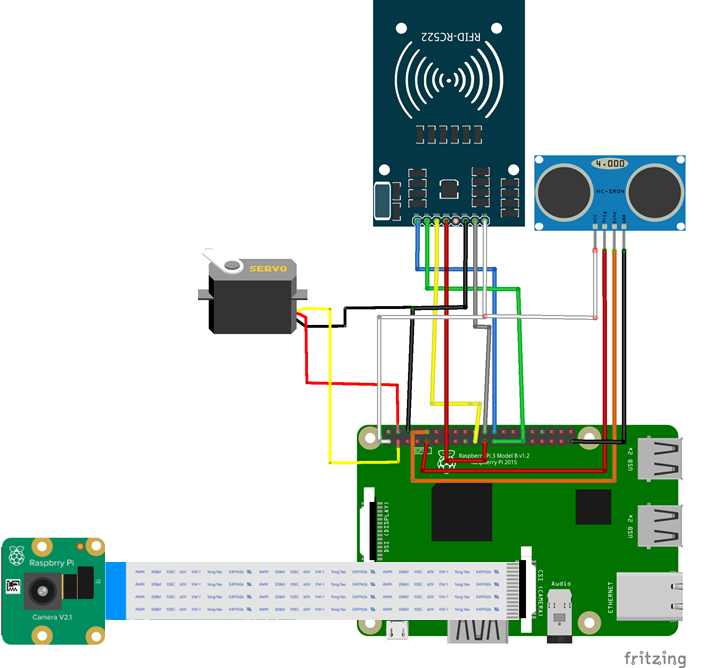
\includegraphics[width=0.85\textwidth, center]{images/skematik-full.png}
    \caption{Rangkaian Skematik Alat}
    \label{fig:rangkaianSkematikAlat}
\end{figure}

\begin{figure} [H]
    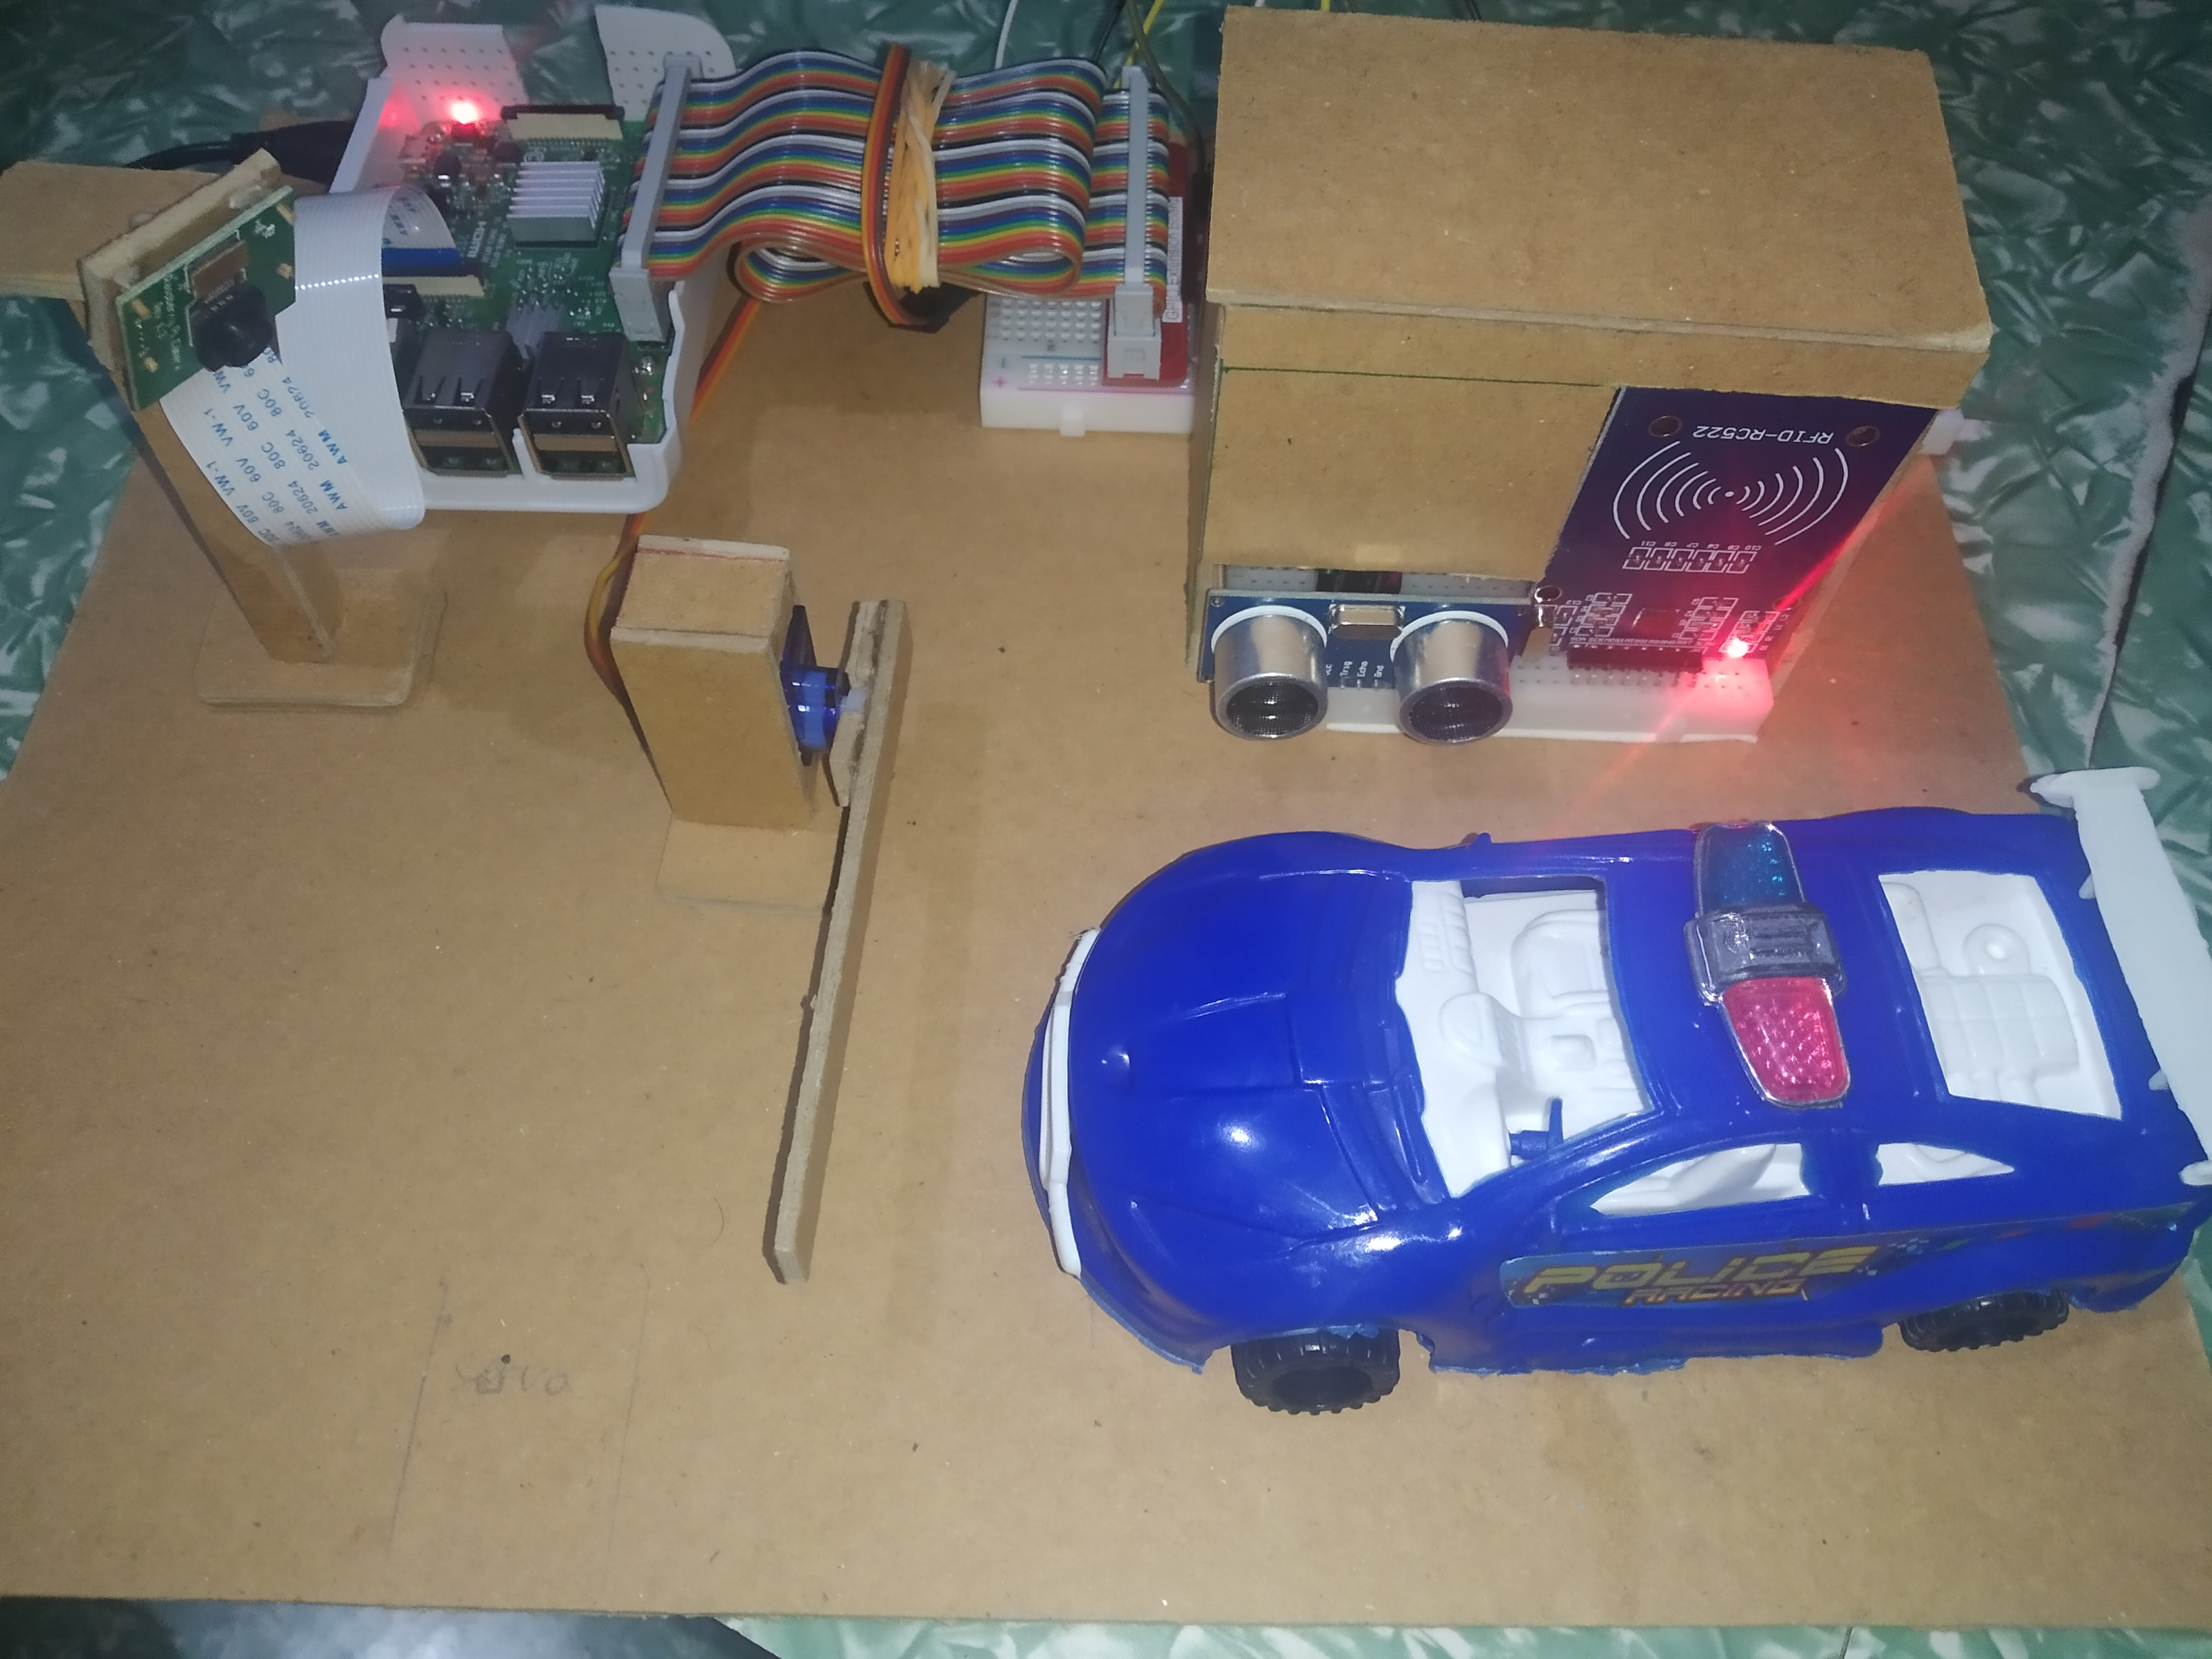
\includegraphics[height=9cm, width=0.85\textwidth, center]{images/alat-full-mobil.jpg}
    \caption{Hasil Rancangan dan Pemasangan Alat}
    \label{fig:alatfullmobil}
\end{figure}

\begin{figure} [H]
    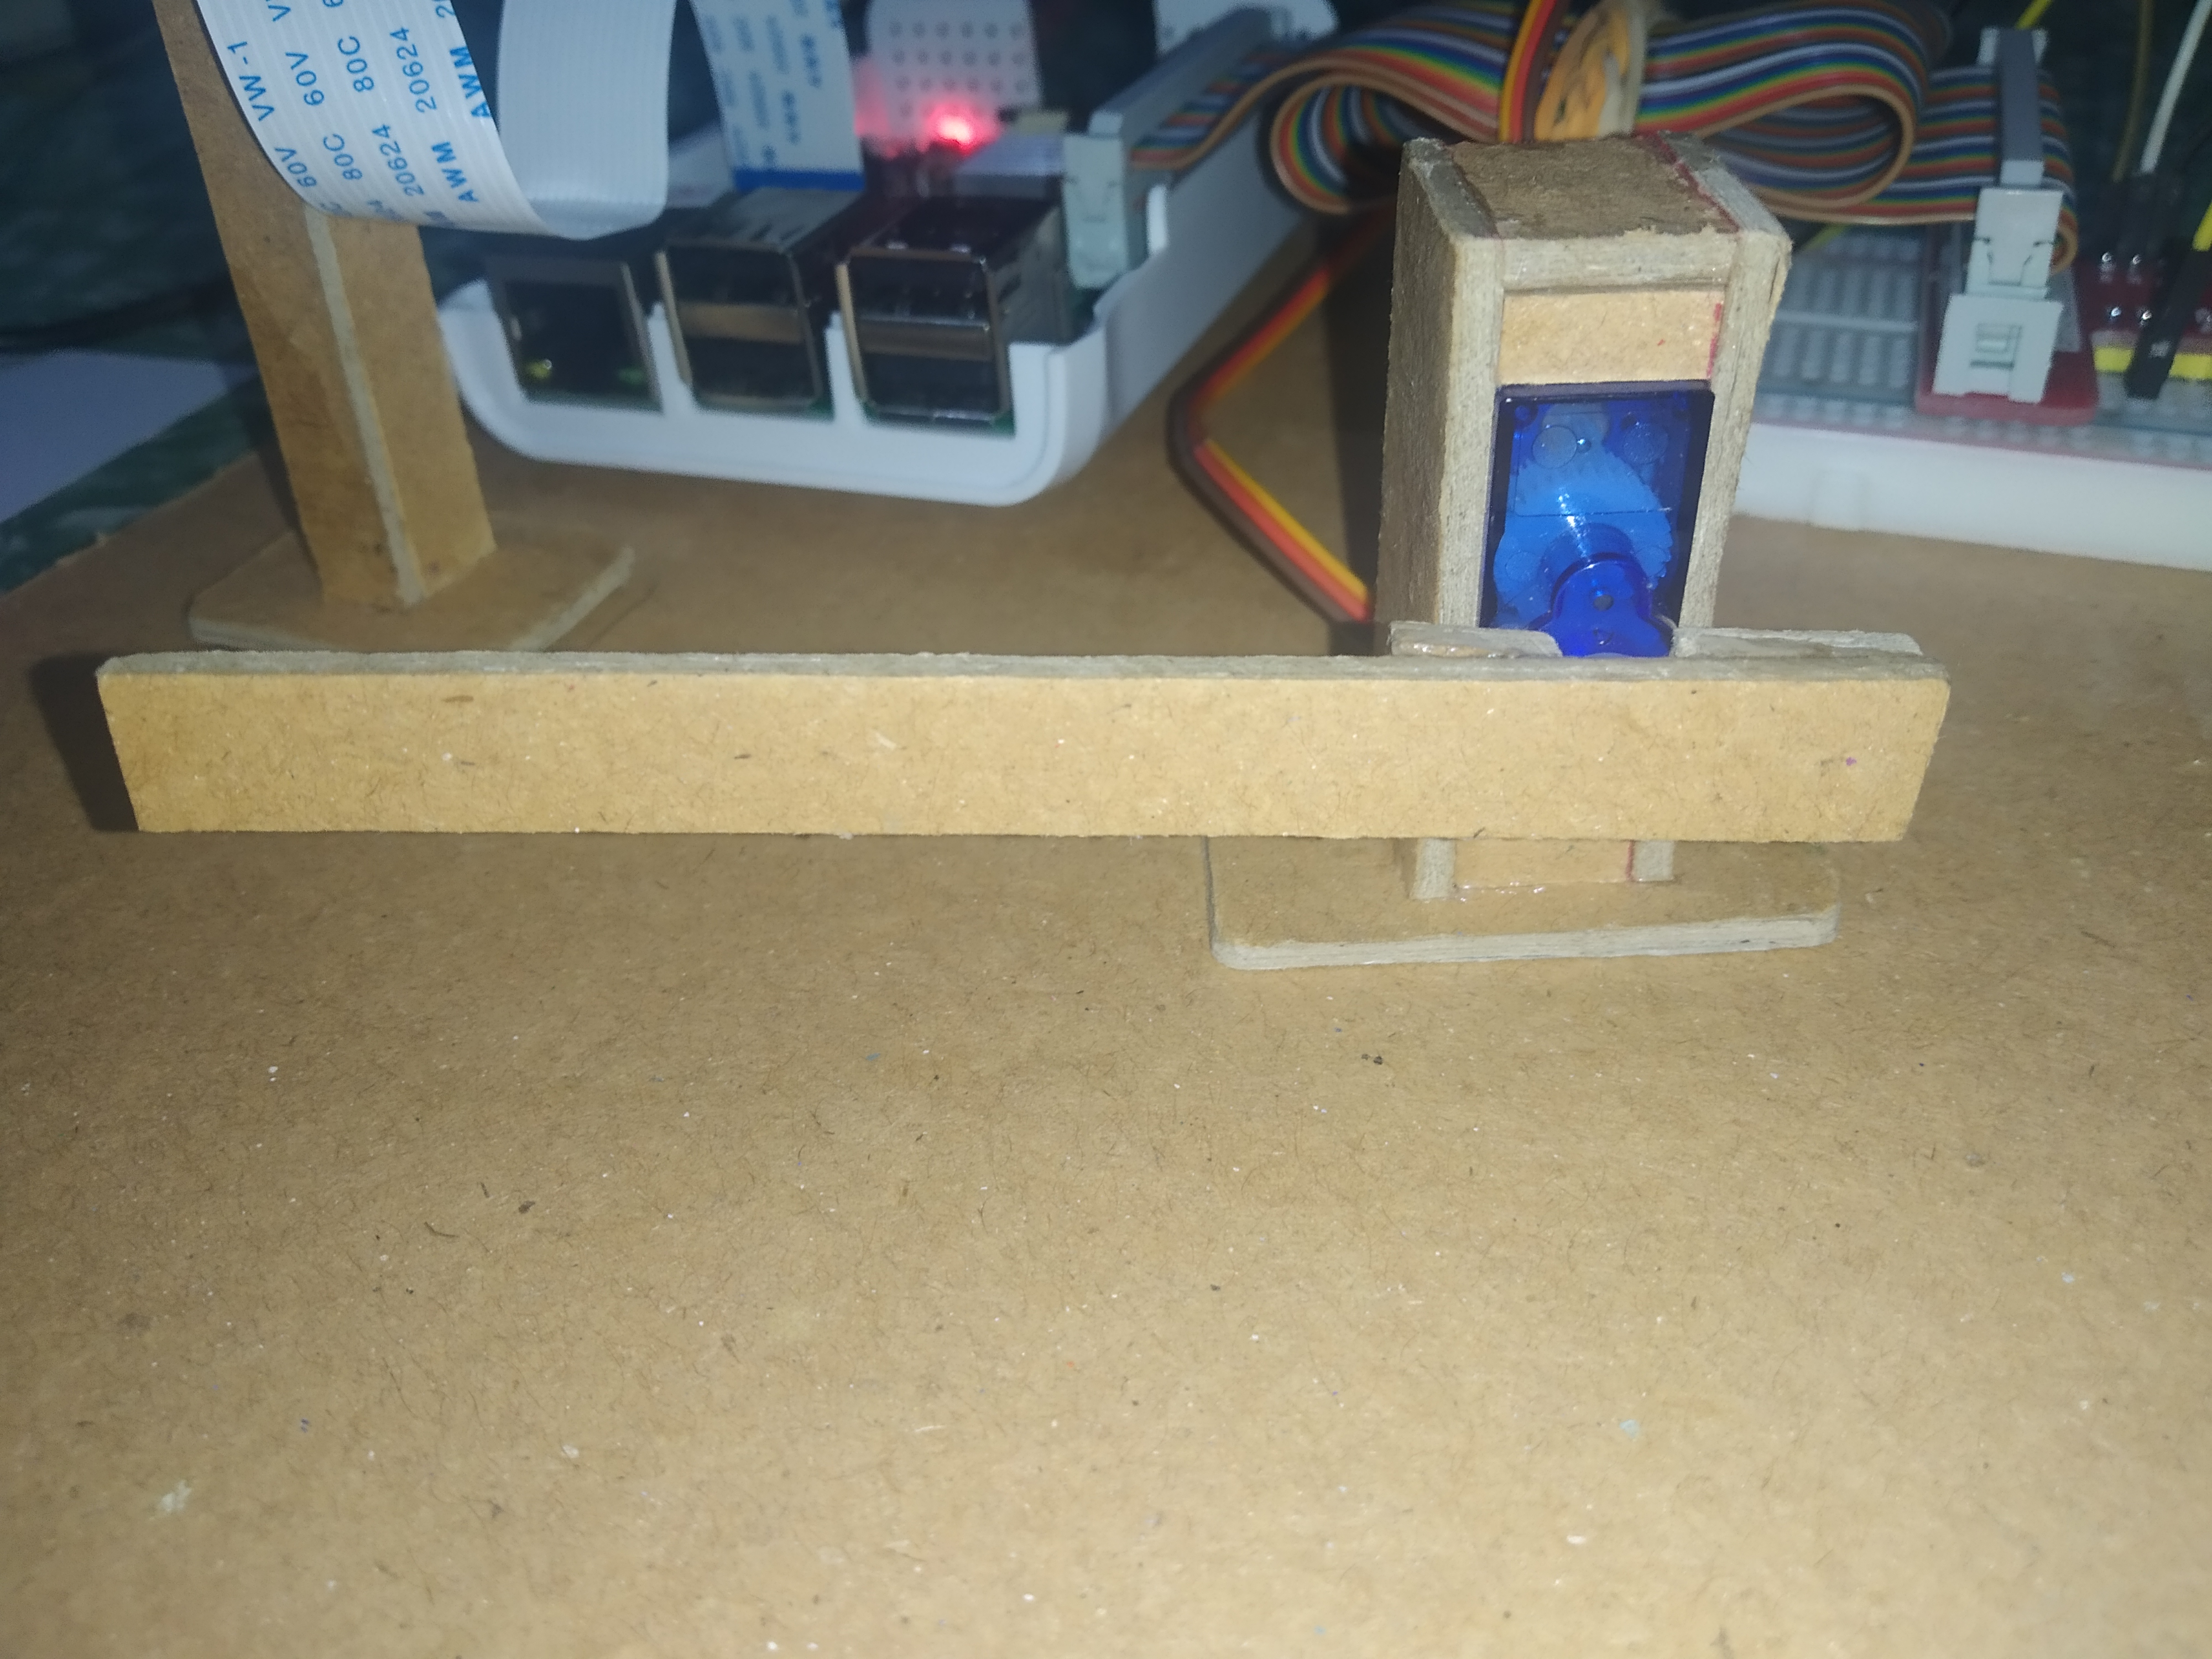
\includegraphics[height=7cm, width=0.5\textwidth, center]{images/alat-servo.jpg}
    \caption{Hasil Rancangan Servo}
    \label{fig:alatservo}
\end{figure}

\begin{figure} [H]
    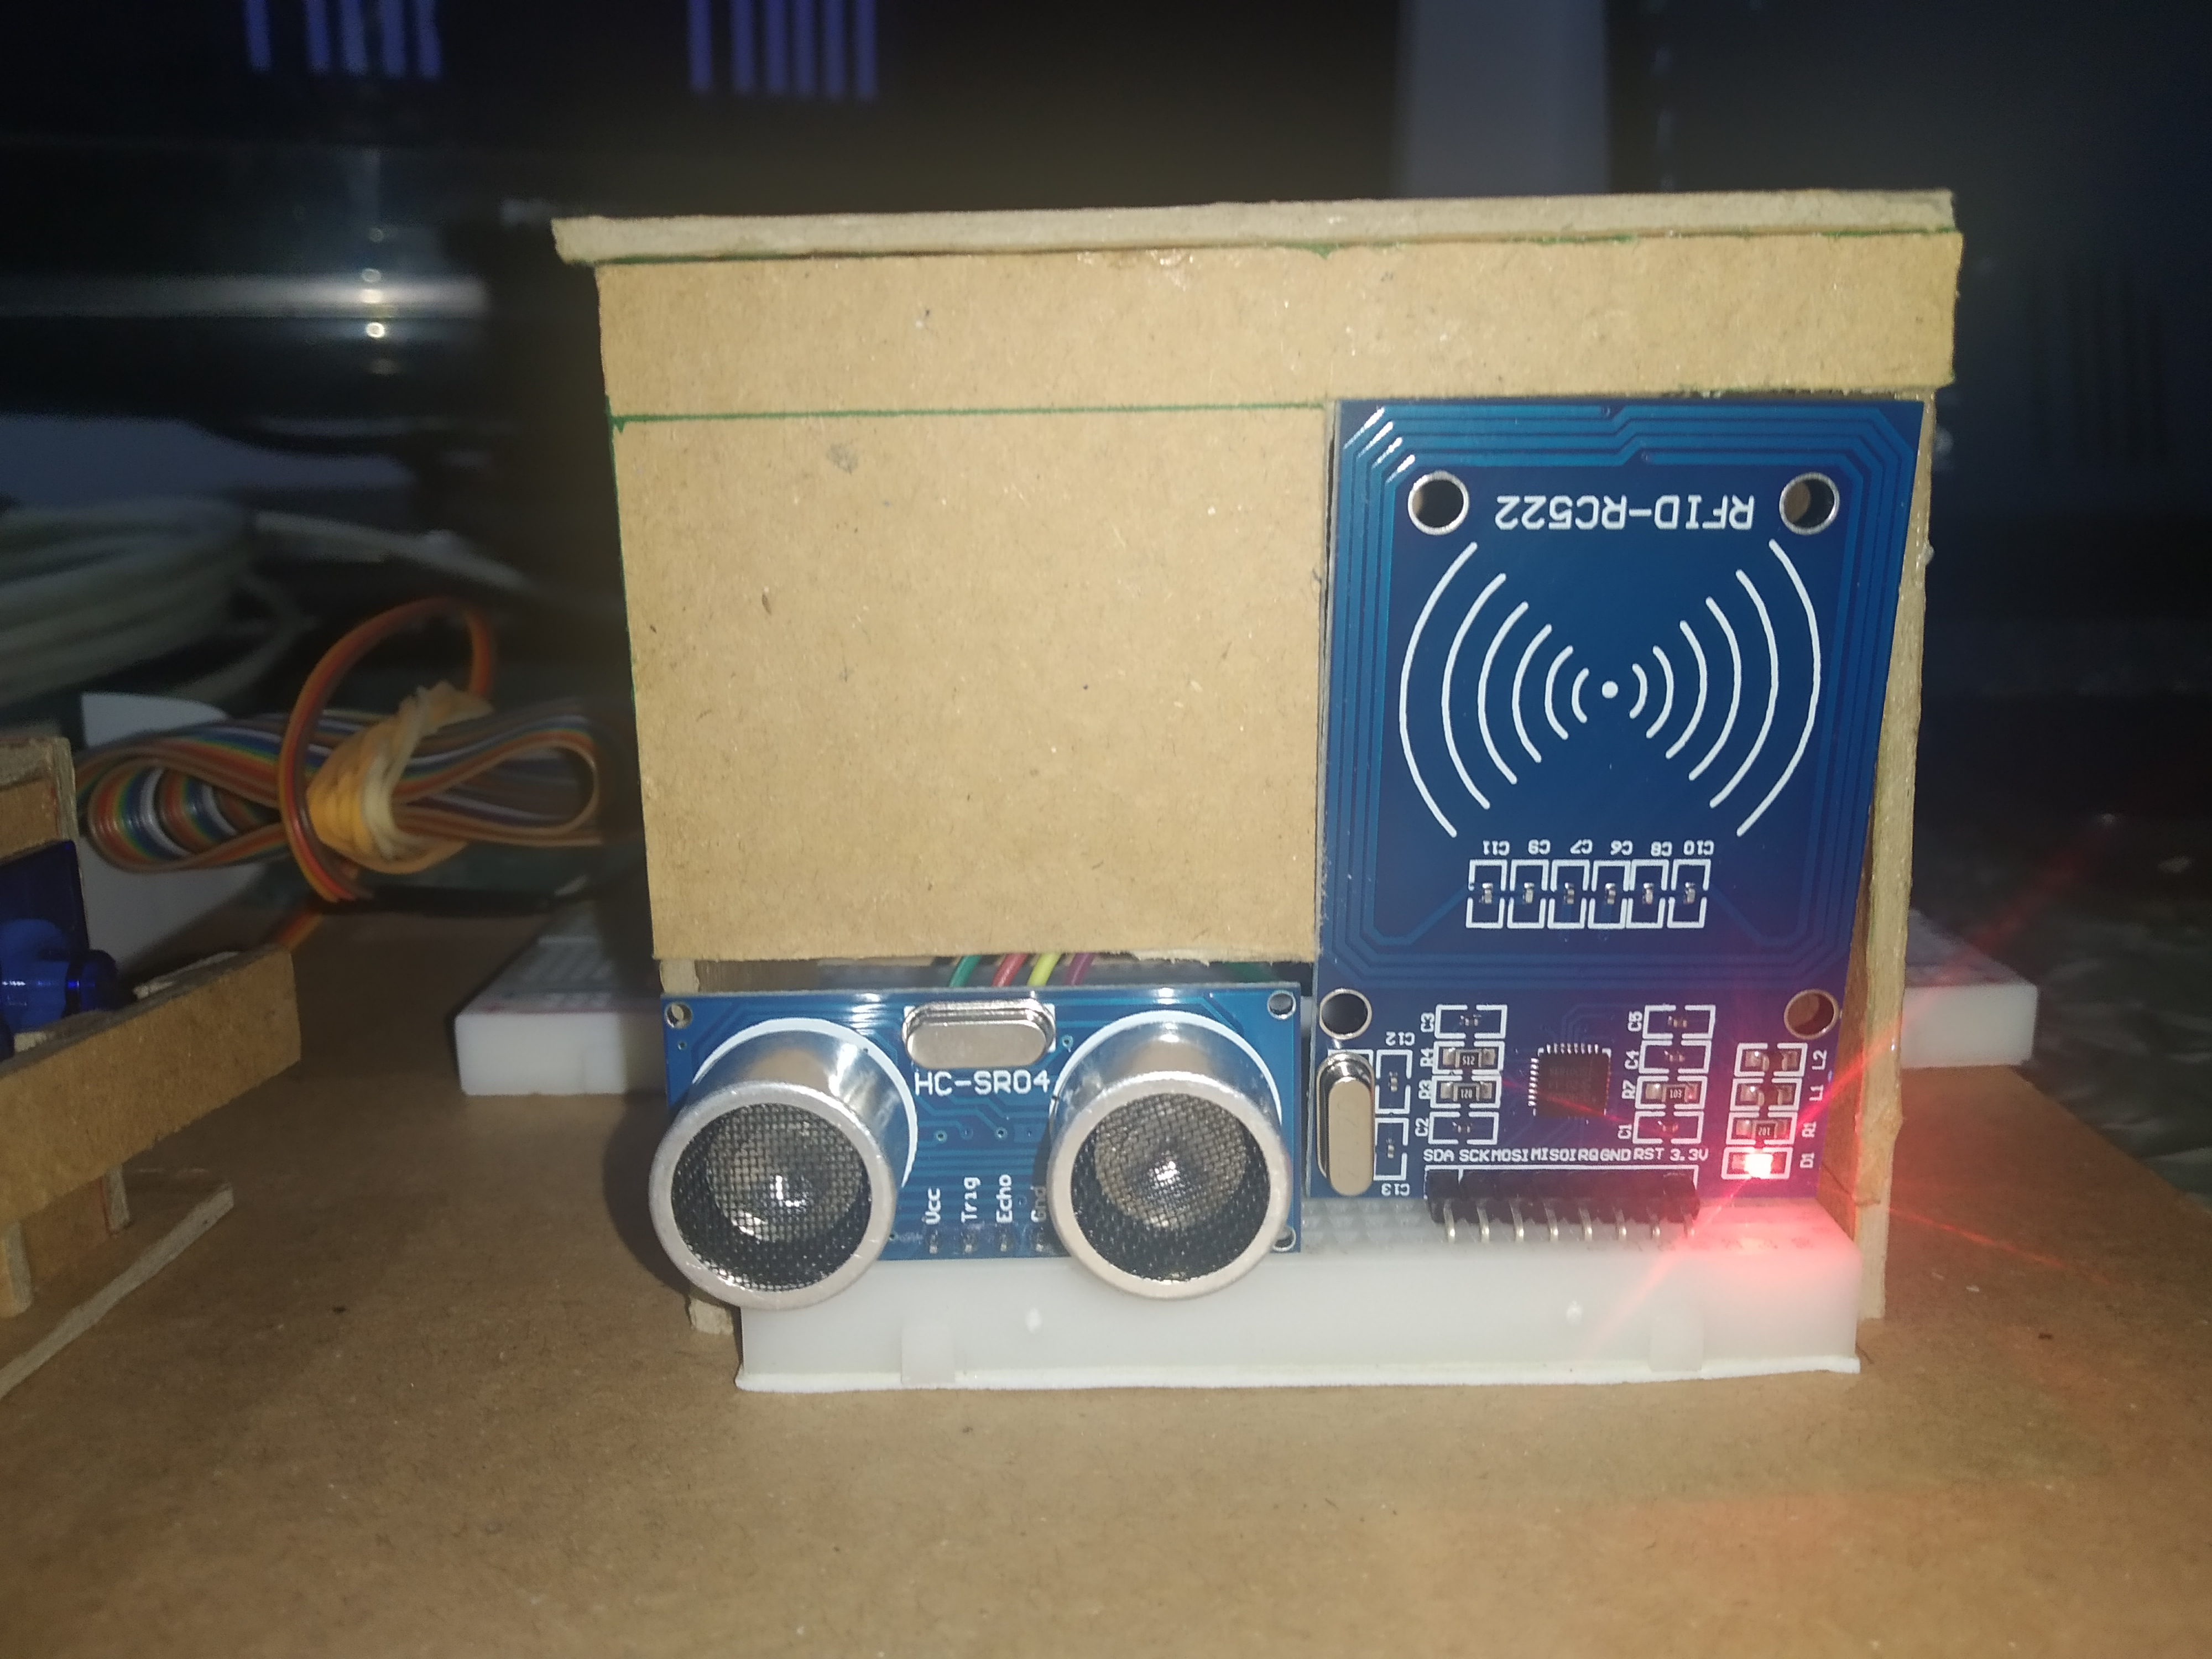
\includegraphics[height=7cm, width=0.65\textwidth, center]{images/alat-ultra&rfid.jpg}
    \caption{Hasil Rancangan Ultrasonik dan RFID}
    \label{fig:alatultrarfid}
\end{figure}

\begin{figure} [H]
    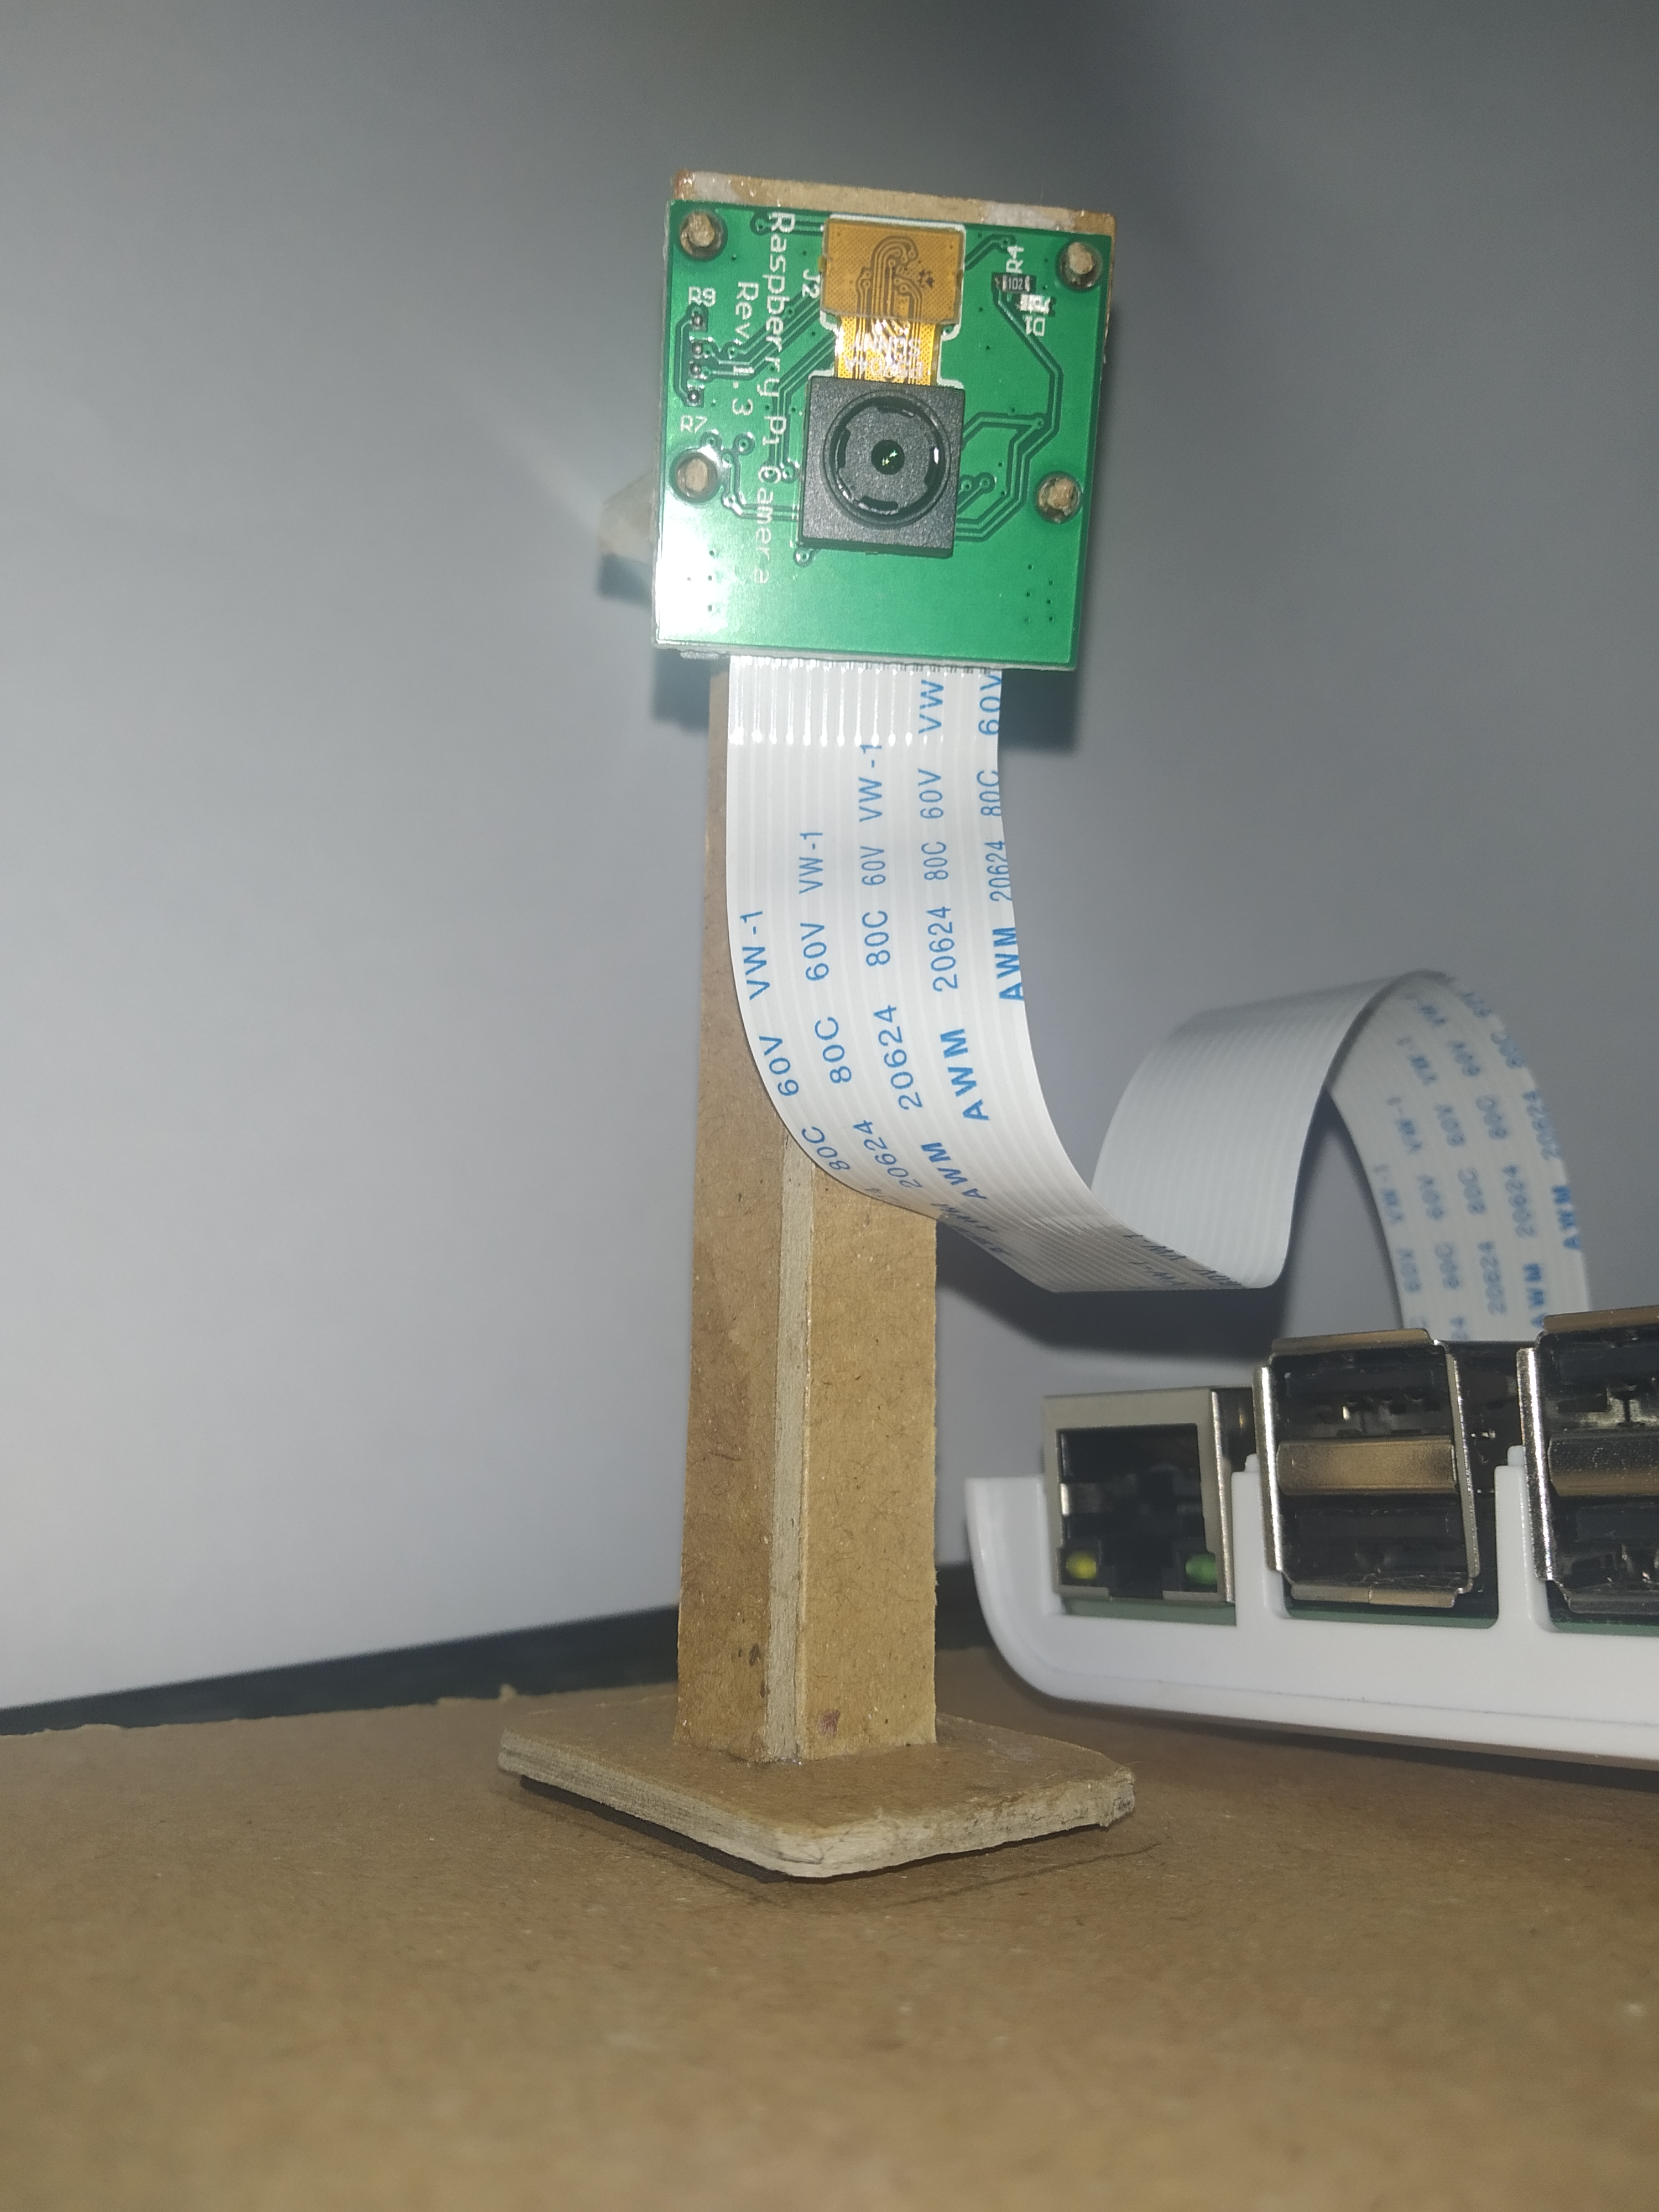
\includegraphics[height=7cm, width=0.5\textwidth, center]{images/alat-kamera.jpg}
    \caption{Hasil Rancangan Kamera}
    \label{fig:alatkamera}
\end{figure}

Pada gambar diatas merupakan rangkaian perangkat keras untuk penelitian di mana seluruh perangkat dirangkai menjadi satu rangkaian.  Gambar ~\ref{fig:alatfullmobil} merupakan hasil dari rancangan dari penelitian yang dilakukan, yang dimana masih bersifat \textit{prototype}. Pada gambar ~\ref{fig:alatservo} dapat dilihat bahwa servo digambarkan sebagai palang parkir. Pada gambar ~\ref{fig:alatultrarfid} dapat dilihat sensor ultrasonik yang akan membaca jarak dari kendaraan untuk menentukan apakah kendaraan masih ada atau sudah tidak ada dan sensor rfid untuk membaca kartu atau tag dari pengendara. Pada gambar ~\ref{fig:alatkamera} dapat dilihat kamera raspberry yang digunakan untuk mengambil nomor plat kendaraan. \textit{Activity} diagram pada sistem yang dibuat bisa dilihat pada gambar ~\ref{fig:diagrammasuk} dan gambar ~\ref{fig:diagramkeluar}.\newline

\begin{figure} [H]
    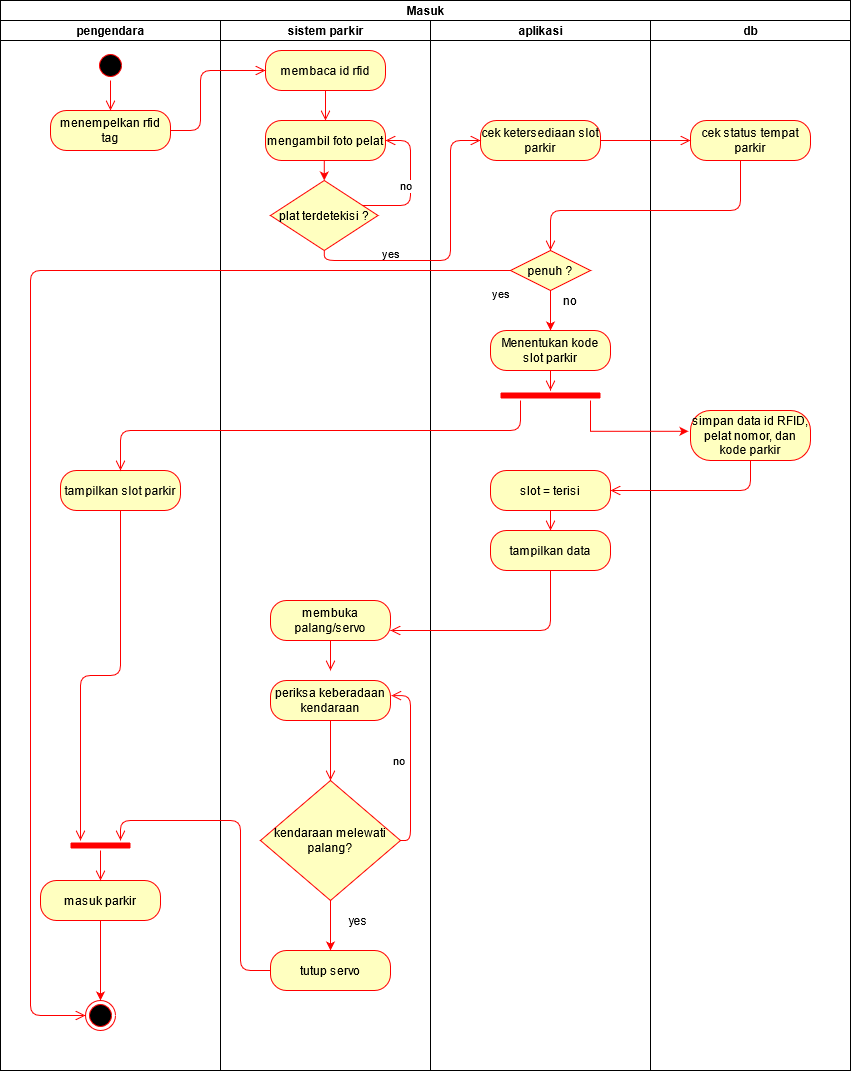
\includegraphics[width=1\textwidth, center]{images/activity diagram skripsi masuk.png}
    \caption{Activity Diagram Masuk}
    \label{fig:diagrammasuk}
\end{figure}

\begin{figure} [H]
    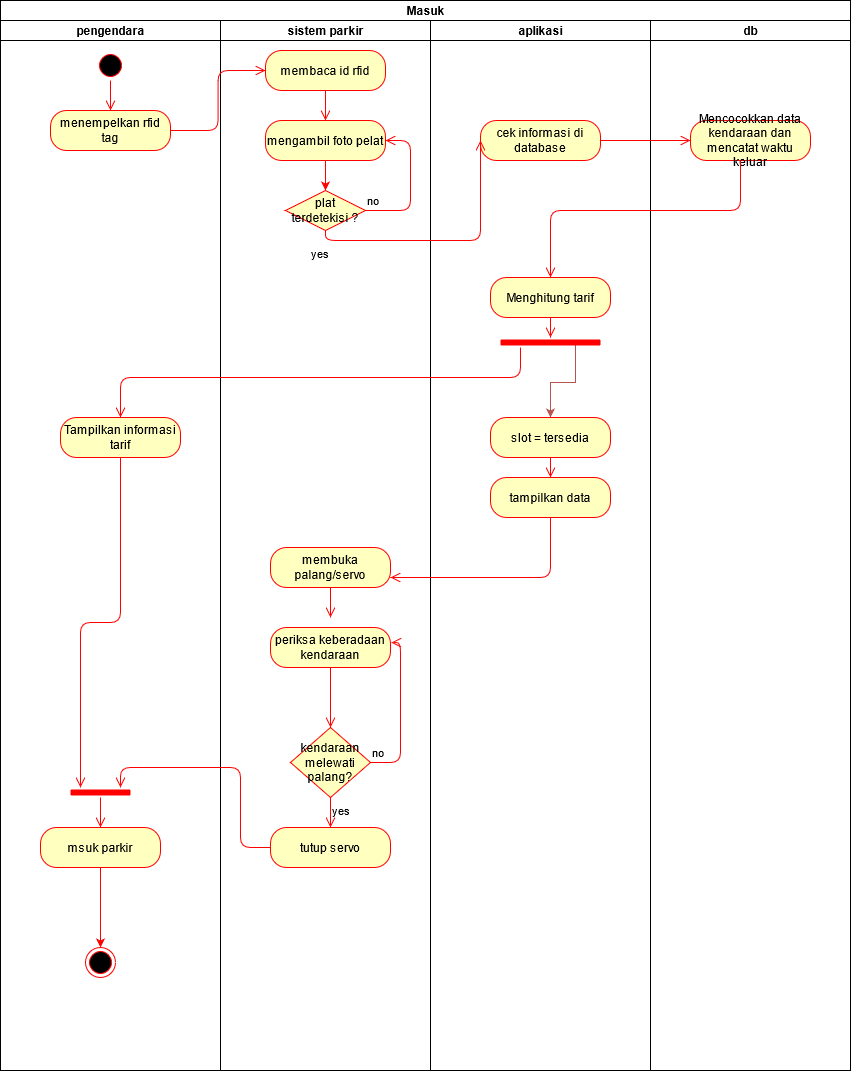
\includegraphics[width=1\textwidth, center]{images/activity diagram skripsi keluar.png}
    \caption{Activity Diagram Keluar}
    \label{fig:diagramkeluar}
\end{figure}

\subsection{Raspberry Pi dan RFID MFRC522}
\begin{figure} [H]
    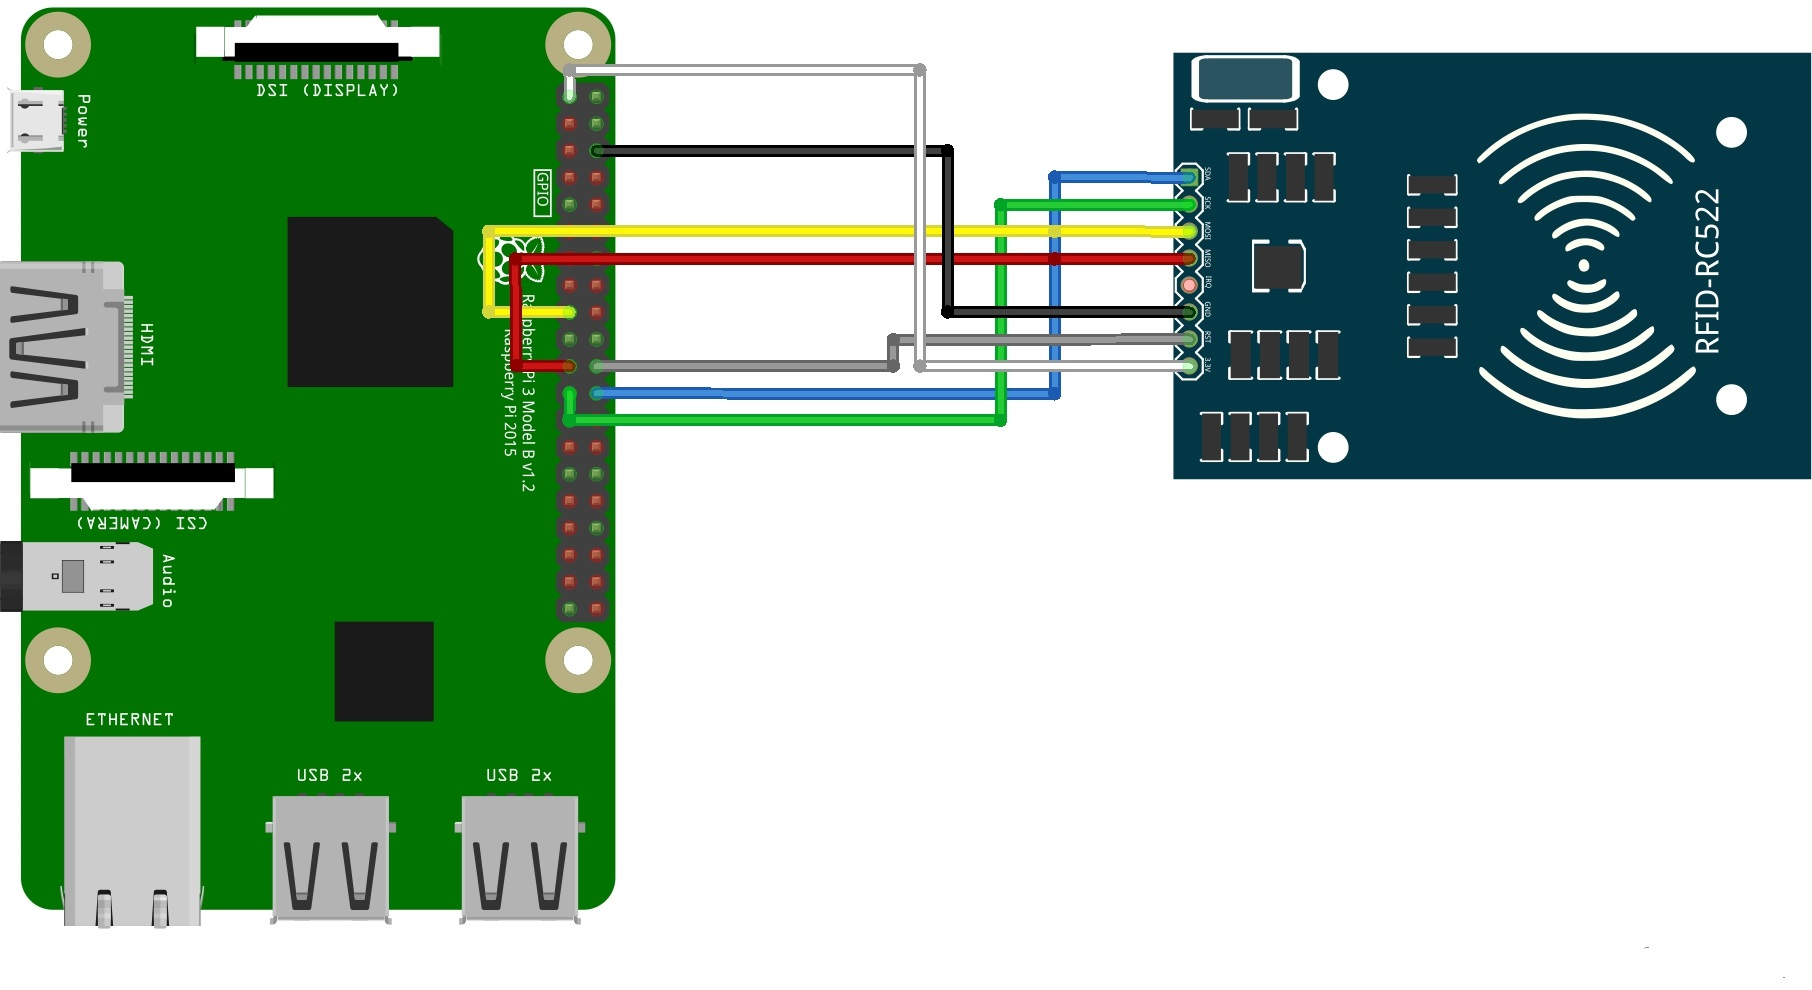
\includegraphics[width=0.85\textwidth, center]{images/skematik_rfid.jpg}
    \caption{Ragkaian Raspberry Pi dan RFID}
    \label{fig:skematikRfid}
\end{figure}

Berdasarkan gambar ~\ref{fig:skematikRfid} Menunjukkan Raspberry Pi sebagai mikrokontroler untuk menghubungkan sensor RFID yang akan membaca kartu atau tag dari pengendara. Untuk pin pada Raspberry Pi dihubungkan pada sensor RFID dapat dilihat pada tabel ~\ref{table:tableRfid}.\newline

\begin{atable}
    \caption{Rangkaian pin RFID ke Raspberry Pi}
    \label{table:tableRfid}
    \csvreader[
        % column count = 11,
        respect underscore=true,
        tabular=cc,
        head to column names,
        before table=\rowcolors{2}{gray!15}{gray!30},
        table head= \rowcolor{gray!50!black} 
            \color{white} RFID & 
            \color{white} RASPBERRY PI 
            \\]
        {tables/tablerfid.csv}
        {
            RFID=\RFID, 
            RASPBERRYPI=\RASPBERRYPI}
        {
            \RFID & 
            \RASPBERRYPI}
\end{atable}

Berikut ini dilakukan pengujian jarak baca kartu RFID yang berfungsi untuk melihat jarak maksimum keterbacaan RFID dari bagian pembaca ke kartu RFID. Pengujian ini dilakukan dengan cara meletakkan kartu RFID dengan memberi jarak tertentu pada area pembacaan. Hasil pengujian dapat dilihat pada tabel ~\ref{table:tableUjiRfid}.

\begin{table}[H]
    \caption{Hasil uji jarak baca RFID}
    \label{table:tableUjiRfid}
    \centering
    \csvreader[
        % column count = 11,
        respect underscore=true,
        tabular=ccc,
        head to column names,
        before table=\rowcolors{2}{gray!15}{gray!30},
        table head= \rowcolor{gray!50!black} 
            \color{white} No. & 
            \color{white} Jarak (mm) & 
            \color{white} Terbaca
            \\]
        {tables/hasil-uji-jarak-rfid.csv}
        {
            No=\No, 
            Jarak=\Jarak,
            Terbaca=\Terbaca}
        {
            \No & 
            \Jarak &
            \Terbaca}
\end{table}

Berdasarkan data hasil pengujian sensor RFID pada tabel ~\ref{table:tableUjiRfid}, pengambilan data dilakukan sebanyak dua puluh kali. Dari data hasil pengukuran yang pertama sampai ke lima belas dengan jarak 0 mm sampai 28 mm, kartu RFID dapat terbaca dengan baik dan pengukuran ke enam belas sampai dua puluh dengan jarak 30 mm sampai 38 mm, kartu sudah tidak bisa tebrbaca.

\subsection{Raspberry Pi dan HC-SR04}
\begin{figure} [H]
    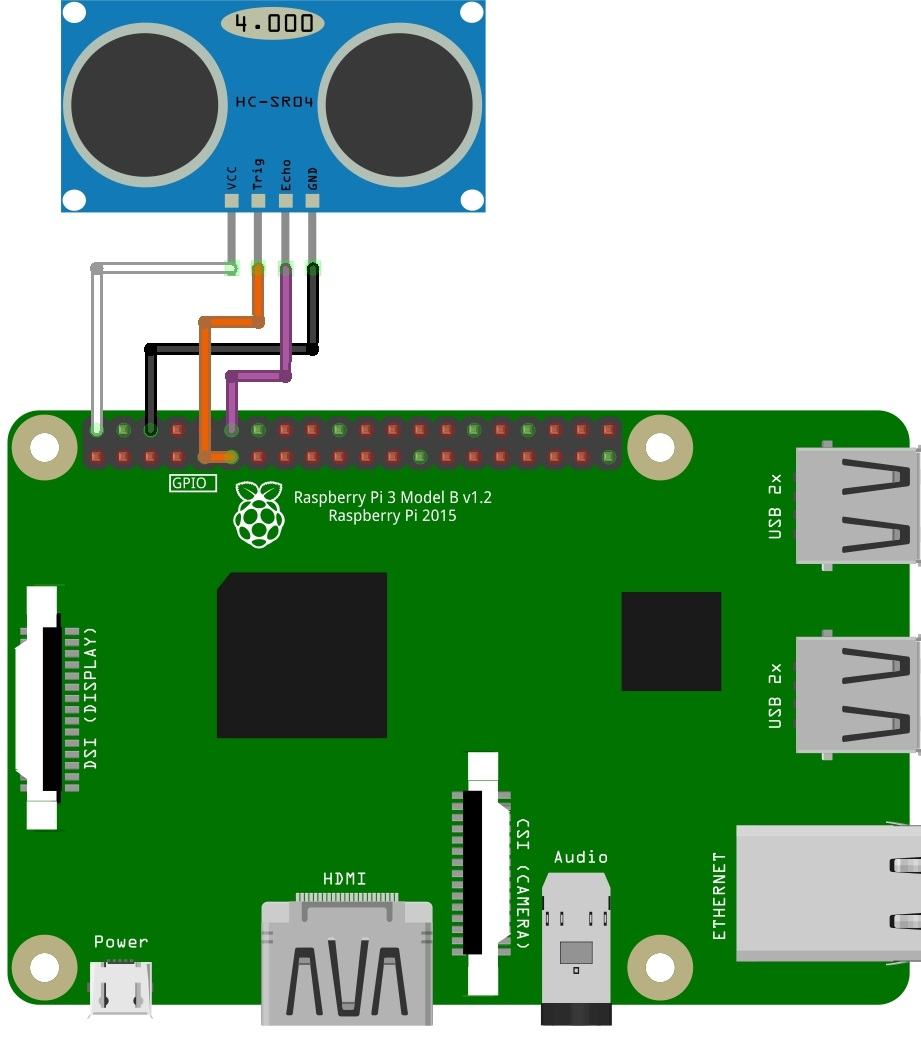
\includegraphics[height=7cm, width=0.5\textwidth, center]{images/skematik_ultra.jpg}
    \caption{Ragkaian Raspberry Pi dan Ultrasonik}
    \label{fig:skematikUltrasonik}
\end{figure}

Gambar ~\ref{fig:skematikUltrasonik} merupakan gambar rangkaian Raspberry Pi dan sensor ultrasonik. Sensor ultrasonik berfungsi sebagai indikator untuk menutup palang parkir. Apabila didepan sensor ultrasonik masih ada kendaraan, maka palang parkir masih akan terbuka, sebaliknya apabila didepan sensor sudah tidak ada kendaraan, maka palang parkir akan menutup. Sensor ultrasonik yang digunakan adalah HC-SR04 yang mempunyai 4 pin yaitu pin \textit{ground} (-), pin \textit{echo}, pin \textit{trigger}, dan pin vcc (+). Untuk pin pada Raspberry Pi dihubungkan pada sensor HC-SR04 dapat dilihat pada tabel ~\ref{table:tableUltrasonic}.\newline

\begin{atable}
    \caption{Rangkaian pin Ultrasonik ke Raspberry Pi}
    \label{table:tableUltrasonic}
    \csvreader[
        % column count = 11,
        respect underscore=true,
        tabular=cc,
        head to column names,
        before table=\rowcolors{2}{gray!15}{gray!30},
        table head= \rowcolor{gray!50!black} 
            \color{white} ULTRASONIK & 
            \color{white} RASPBERRY PI 
            \\]
        {tables/tableultrasonic.csv}
        {
            ULTRASONIC=\ULTRASONIC, 
            RASPBERRYPI=\RASPBERRYPI}
        {
            \ULTRASONIC & 
            \RASPBERRYPI}
\end{atable}

Berikut ini pengujian yang dilakukan pada sensor ultrasonik untuk mengukur tinggat kesalahan jarak yang diukur oleh sensor ultrasonik dibandingkan jarak sebenarnya dengan pengukuran secara manual: \newline \newline

% \begin{table}[H]
%     \caption{Hasil uji jarak baca servo}
%     \label{table:tableUjiServo}
%     \begin{tabular}{cccccccccc}
%     \hline
%     \multirow{3}{*}{\begin{tabular}[c]{@{}c@{}}Pengukuran \\ Manual\end{tabular}} & \multicolumn{3}{c}{\begin{tabular}[c]{@{}c@{}}Pengukuran \\ Sensor (cm)\end{tabular}} & \multicolumn{3}{c}{\begin{tabular}[c]{@{}c@{}}Selisih \\ Pengukuran (cm)\end{tabular}} & \multicolumn{3}{c}{\begin{tabular}[c]{@{}c@{}}Persentase \\ Kesalahan(\%)\end{tabular}} \\ \cline{2-10} 
%                                                                                   & \multicolumn{3}{c|}{Pengukuran ke-}                                                   & \multicolumn{3}{c|}{Pengukuran ke-}                                                    & \multicolumn{3}{c|}{Pengukuran ke-}                                                     \\ \cline{2-10} 
%                                                                                   & \multicolumn{1}{c|}{1}      & \multicolumn{1}{c|}{2}     & \multicolumn{1}{c|}{3}     & \multicolumn{1}{c|}{1}      & \multicolumn{1}{c|}{2}      & \multicolumn{1}{c|}{3}     & \multicolumn{1}{c|}{1}      & \multicolumn{1}{c|}{2}      & \multicolumn{1}{c|}{3}      \\ \hline
%     \multicolumn{1}{|c|}{2}                                                       & \multicolumn{1}{c|}{2}      & \multicolumn{1}{c|}{2}     & \multicolumn{1}{c|}{2}     & \multicolumn{1}{c|}{0}      & \multicolumn{1}{c|}{0}      & \multicolumn{1}{c|}{0}     & \multicolumn{1}{c|}{0}      & \multicolumn{1}{c|}{0}      & \multicolumn{1}{c|}{0}      \\ \hline
%     \multicolumn{1}{|c|}{6}                                                       & \multicolumn{1}{c|}{6}      & \multicolumn{1}{c|}{6}     & \multicolumn{1}{c|}{6}     & \multicolumn{1}{c|}{0}      & \multicolumn{1}{c|}{0}      & \multicolumn{1}{c|}{0}     & \multicolumn{1}{c|}{0}      & \multicolumn{1}{c|}{0}      & \multicolumn{1}{c|}{0}      \\ \hline
%     \multicolumn{1}{|c|}{15}                                                      & \multicolumn{1}{c|}{15}     & \multicolumn{1}{c|}{15}    & \multicolumn{1}{c|}{15}    & \multicolumn{1}{c|}{0}      & \multicolumn{1}{c|}{0}      & \multicolumn{1}{c|}{0}     & \multicolumn{1}{c|}{0}      & \multicolumn{1}{c|}{0}      & \multicolumn{1}{c|}{0}      \\ \hline
%     \multicolumn{1}{|c|}{20}                                                      & \multicolumn{1}{c|}{20}     & \multicolumn{1}{c|}{19}    & \multicolumn{1}{c|}{19}    & \multicolumn{1}{c|}{0}      & \multicolumn{1}{c|}{1}      & \multicolumn{1}{c|}{1}     & \multicolumn{1}{c|}{0}      & \multicolumn{1}{c|}{5}      & \multicolumn{1}{c|}{5}      \\ \hline
%     \multicolumn{1}{|c|}{30}                                                      & \multicolumn{1}{c|}{29}     & \multicolumn{1}{c|}{29}    & \multicolumn{1}{c|}{29}    & \multicolumn{1}{c|}{1}      & \multicolumn{1}{c|}{1}      & \multicolumn{1}{c|}{1}     & \multicolumn{1}{c|}{3}      & \multicolumn{1}{c|}{3}      & \multicolumn{1}{c|}{3}      \\ \hline
%     \multicolumn{1}{|c|}{40}                                                      & \multicolumn{1}{c|}{38}     & \multicolumn{1}{c|}{39}    & \multicolumn{1}{c|}{38}    & \multicolumn{1}{c|}{2}      & \multicolumn{1}{c|}{1}      & \multicolumn{1}{c|}{2}     & \multicolumn{1}{c|}{5}      & \multicolumn{1}{c|}{3}      & \multicolumn{1}{c|}{5}      \\ \hline
%     \multicolumn{1}{|c|}{50}                                                      & \multicolumn{1}{c|}{49}     & \multicolumn{1}{c|}{49}    & \multicolumn{1}{c|}{49}    & \multicolumn{1}{c|}{1}      & \multicolumn{1}{c|}{1}      & \multicolumn{1}{c|}{1}     & \multicolumn{1}{c|}{2}      & \multicolumn{1}{c|}{2}      & \multicolumn{1}{c|}{2}      \\ \hline
%     \multicolumn{1}{|c|}{60}                                                      & \multicolumn{1}{c|}{57}     & \multicolumn{1}{c|}{56}    & \multicolumn{1}{c|}{57}    & \multicolumn{1}{c|}{3}      & \multicolumn{1}{c|}{4}      & \multicolumn{1}{c|}{3}     & \multicolumn{1}{c|}{5}      & \multicolumn{1}{c|}{7}      & \multicolumn{1}{c|}{5}      \\ \hline
%     \multicolumn{1}{|c|}{70}                                                      & \multicolumn{1}{c|}{68}     & \multicolumn{1}{c|}{69}    & \multicolumn{1}{c|}{68}    & \multicolumn{1}{c|}{2}      & \multicolumn{1}{c|}{1}      & \multicolumn{1}{c|}{2}     & \multicolumn{1}{c|}{3}      & \multicolumn{1}{c|}{1}      & \multicolumn{1}{c|}{3}      \\ \hline
%     \multicolumn{1}{|c|}{80}                                                      & \multicolumn{1}{c|}{78}     & \multicolumn{1}{c|}{78}    & \multicolumn{1}{c|}{78}    & \multicolumn{1}{c|}{2}      & \multicolumn{1}{c|}{2}      & \multicolumn{1}{c|}{2}     & \multicolumn{1}{c|}{3}      & \multicolumn{1}{c|}{3}      & \multicolumn{1}{c|}{3}      \\ \hline
%     \multicolumn{1}{|c|}{90}                                                      & \multicolumn{1}{c|}{89}     & \multicolumn{1}{c|}{90}    & \multicolumn{1}{c|}{88}    & \multicolumn{1}{c|}{1}      & \multicolumn{1}{c|}{0}      & \multicolumn{1}{c|}{2}     & \multicolumn{1}{c|}{1}      & \multicolumn{1}{c|}{0}      & \multicolumn{1}{c|}{2}      \\ \hline
%     \multicolumn{1}{|c|}{100}                                                     & \multicolumn{1}{c|}{96}     & \multicolumn{1}{c|}{97}    & \multicolumn{1}{c|}{96}    & \multicolumn{1}{c|}{4}      & \multicolumn{1}{c|}{3}      & \multicolumn{1}{c|}{4}     & \multicolumn{1}{c|}{4}      & \multicolumn{1}{c|}{3}      & \multicolumn{1}{c|}{4}      \\ \hline
%     \multicolumn{1}{|c|}{110}                                                     & \multicolumn{1}{c|}{107}    & \multicolumn{1}{c|}{107}   & \multicolumn{1}{c|}{108}   & \multicolumn{1}{c|}{3}      & \multicolumn{1}{c|}{3}      & \multicolumn{1}{c|}{2}     & \multicolumn{1}{c|}{3}      & \multicolumn{1}{c|}{3}      & \multicolumn{1}{c|}{2}      \\ \hline
%     \multicolumn{1}{|c|}{120}                                                     & \multicolumn{1}{c|}{115}    & \multicolumn{1}{c|}{114}   & \multicolumn{1}{c|}{115}   & \multicolumn{1}{c|}{5}      & \multicolumn{1}{c|}{6}      & \multicolumn{1}{c|}{5}     & \multicolumn{1}{c|}{4}      & \multicolumn{1}{c|}{5}      & \multicolumn{1}{c|}{4}      \\ \hline
%     \multicolumn{7}{c}{Rata-rata kesalahan}                                                                                                                                                                                                                        & 2,34                        & 2,44                        & 2,71                        \\ \hline
%     \end{tabular}
% \end{table}

\begin{atable} 
    \caption{Hasil uji jarak baca servo}
    \label{table:tableUjiServo}
    \begin{tabular}{|c|c|c|c|c|c|c|c|c|c|}
    \hline
    \multirow{3}{2cm}{Pengukuran Manual(cm)} & \multicolumn{3}{c|}{Pengukuran Sensor(cm)} & \multicolumn{3}{c|}{Selisih Pengukuran(cm)} & \multicolumn{3}{c|}{Persentase Kesalahan(\%)} \\ \cline{2-10} 
                                       & \multicolumn{3}{c|}{Pengukuran ke-}         & \multicolumn{3}{c|}{Pengukuran ke-}          & \multicolumn{3}{c|}{Pengukuran ke-}       \\ \cline{2-10} 
                                       & 1             & 2            & 3            & 1             & 2             & 3            & 1            & 2            & 3           \\ \hline
    2                                  & 2             & 2            & 2            & 0             & 0             & 0            & 0            & 0            & 0           \\ \hline
    6                                  & 6             & 6            & 6            & 0             & 0             & 0            & 0            & 0            & 0           \\ \hline
    15                                 & 15            & 15           & 15           & 0             & 0             & 0            & 0            & 0            & 0           \\ \hline
    20                                 & 20            & 19           & 19           & 0             & 1             & 1            & 0            & 5            & 5           \\ \hline
    30                                 & 29            & 29           & 29           & 1             & 1             & 1            & 3            & 3            & 3           \\ \hline
    40                                 & 38            & 39           & 38           & 2             & 1             & 2            & 5            & 3            & 5           \\ \hline
    50                                 & 49            & 49           & 49           & 1             & 1             & 1            & 2            & 2            & 2           \\ \hline
    60                                 & 57            & 56           & 57           & 3             & 4             & 3            & 5            & 7            & 5           \\ \hline
    70                                 & 68            & 69           & 68           & 2             & 1             & 2            & 3            & 1            & 3           \\ \hline
    80                                 & 78            & 78           & 78           & 2             & 2             & 2            & 3            & 3            & 3           \\ \hline
    90                                 & 89            & 90           & 88           & 1             & 0             & 2            & 1            & 0            & 2           \\ \hline
    100                                & 96            & 97           & 96           & 4             & 3             & 4            & 4            & 3            & 4           \\ \hline
    110                                & 107           & 107          & 108          & 3             & 3             & 2            & 3            & 3            & 2           \\ \hline
    120                                & 115           & 114          & 115          & 5             & 6             & 5            & 4            & 5            & 4           \\ \hline
    \multicolumn{7}{|c|}{Rata-rata kesalahan}                                                                                       & 2,34         & 2,44         & 2,71        \\ \hline
    \end{tabular}
\end{atable}

Berdasarkan data hasil pengujian sensor ultrasonik pada tabel ~\ref{table:tableUjiServo}, pengambilan data dilakukan sebanyak empat belas kali dengan tiga kali pengukuran, didapatkan hasil yang berbeda antara pengukuran manual yang menggunakan penggaris dengan pengukuran oleh sensor. Dari data hasil pengukuran yang pertama didapatbahwa terdapat selisih jarak hasil pengujian oleh sensor dengan jarak sebenarnya, dilakukan pengukuran dengan rentang jarak dari 2 cm sampai 120 cm yang dimana untuk pengukuran 2 cm sampai 15 cm tidak ada selisih antara pengukuran manual dan pengukuran sensor. Pada jarak 20 cm tidak ada selisih untuk pengukuran pertama, sedangkan pengukuran kedua dan ketiga terdapat selisih sebesar 1 cm. Pada jarak 30 cm terdapat selisih 1 cm untuk semua pengukuran. Pada jarak 40 cm selisih pada pengukuran pertama sebesar 2 cm, kedua sebesar 1 cm, dan ketiga sebesar 2 cm. Pada jarak 50 cm dan 60 cm terdapat selisih sebesar 2 cm pada setiap pengukuran. Pada jara 70 cm selisih pada pengukuran pertama sebesar 2 cm, kedua sebesar 1 cm, dan ketiga sebesar 2 cm. Pada jarak 80 cm dan 90 cm terdapat selisih sebesar 3 cm pada setiap pengukuran. Pada jarak 100 cm dan 110 cm terdapat selisih sebesar 4 cm pada setiap pengukuran. Pada jarak 120 cm selisih pada pengukuran pertama sebesar 5 cm, kedua sebesar 6 cm, dan ketiga sebesar 5 cm.

Berdasarkan data hasil pengujian pada tabel menunjukan bahwa semakin jauh jarak yang diukur, semakin besar kesalahan jarak yang diukur oleh sensor dari jarak sebenarnya. Perbedaan jarak hasil pengujian sensor dengan jarak sesungguhnya dapat disebabkan oleh adanya \textit{noise} atau permukaan jarak yang diukur tidak rata.

Berikut ini rumus serta perhitungan yang digunakan untuk menghitungpersentase kesalahan dan rata-rata kesalahan, dari perbandingan pengukuran jarakantara sensor dengan manual:

\begin{enumerate}[topsep=0pt,itemsep=0pt,partopsep=0pt, parsep=0pt]
    \item Persentase kesalahan
    \begin{equation}
        \label{eq:persentase-kesalahan}
        \begin{split}
        \%kesalahan = \frac{(jarak manual - jarak sensor)}{jarak manual} x 100\%
        \end{split}
    \end{equation}

    \item Rata-rata kesalahan
    \begin{equation}
        \label{eq:persentase-kesalahan}
        \begin{split}
        \%rata-rata kesalahan = \frac{jarak \% kesalahan}{banyaknya data} 
        \end{split}
    \end{equation}
\end{enumerate}

\subsection{Raspberry Pi dan SG90}
\begin{figure} [H]
    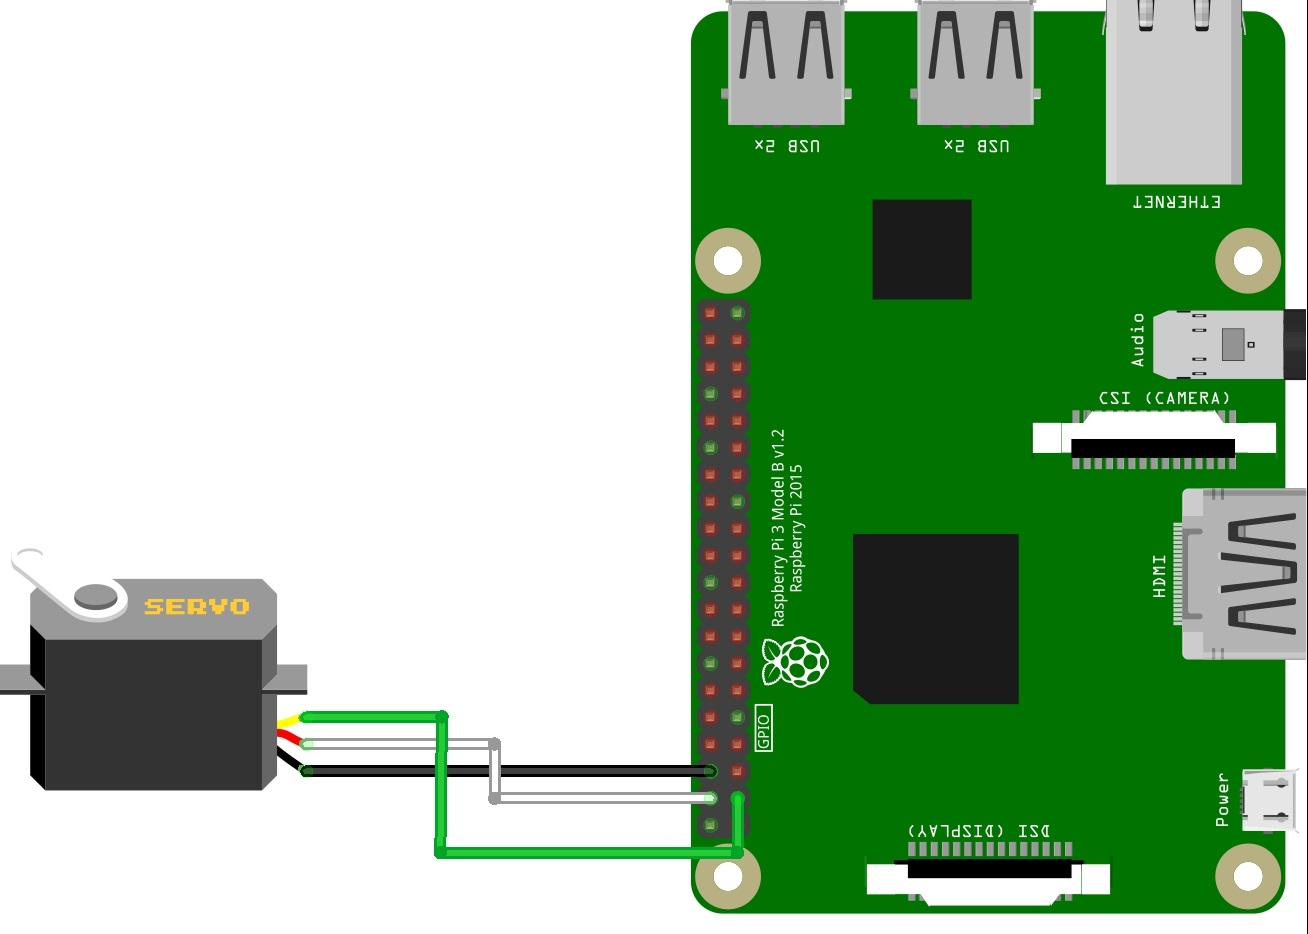
\includegraphics[height=7cm, width=0.6\textwidth, center]{images/skematik_servo.jpg}
    \caption{Ragkaian Raspberry Pi dan Servo}
    \label{fig:skematikServo}
\end{figure}

Pada penelitian ini yang akan berfungsi sebagai palang parkir adalah servo SG90. Servo yang digunakan mempunyai 3 pin yaitu pin \textit{ground} (-), pin pwm, dan pin 5v (+). Untuk pin pada Raspberry Pi dihubungkan pada servo SG90 dapat dilihat pada tabel ~\ref{table:tableServo}.

\begin{atable}
    \caption{Rangkaian pin Servo ke Raspberry Pi}
    \label{table:tableServo}
    \csvreader[
        % column count = 11,
        respect underscore=true,
        tabular=cc,
        head to column names,
        before table=\rowcolors{2}{gray!15}{gray!30},
        table head= \rowcolor{gray!50!black} 
            \color{white} SERVO & 
            \color{white} RASPBERRY PI 
            \\]
        {tables/tableservo.csv}
        {
            SERVO=\SERVO, 
            RASPBERRYPI=\RASPBERRYPI}
        {
            \SERVO & 
            \RASPBERRYPI}
\end{atable}

\subsection{Raspberry Pi dan Kamera Pi}
\begin{figure} [H]
    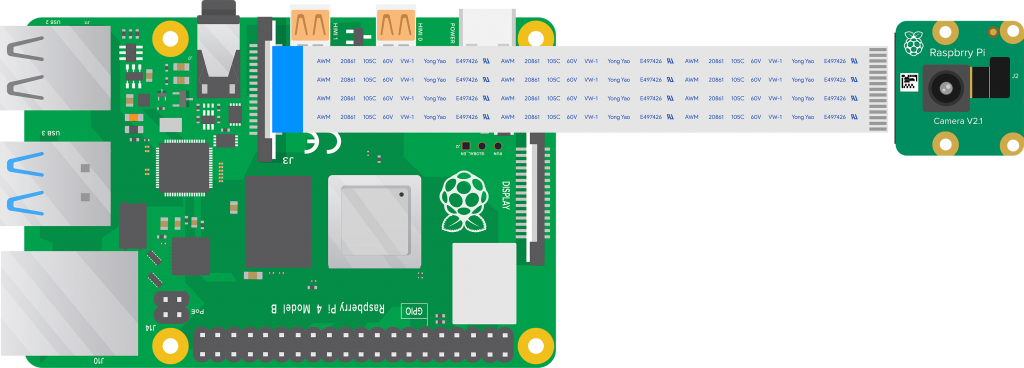
\includegraphics[width=0.85\textwidth, center]{images/skematik-kamera.png}
    \caption{Ragkaian Raspberry Pi dan Kamera}
    \label{fig:skematikKamera}
\end{figure}

Gambar ~\ref{fig:skematikKamera} merupakan gambar skematik Raspberry Pi dengan kamera. Untuk menghubungkan Raspberry Pi dengan kamera cukup dengan menghubungkan kamera dengan port \textit{Camera Serial Interface} (CSI) yang sudah tersedia pada Raspberry Pi. Gambar ~\ref{fig:GambarKameraPi} merupakah hasil foto yang diambil oleh kamera Pi.

\begin{figure} [H]
    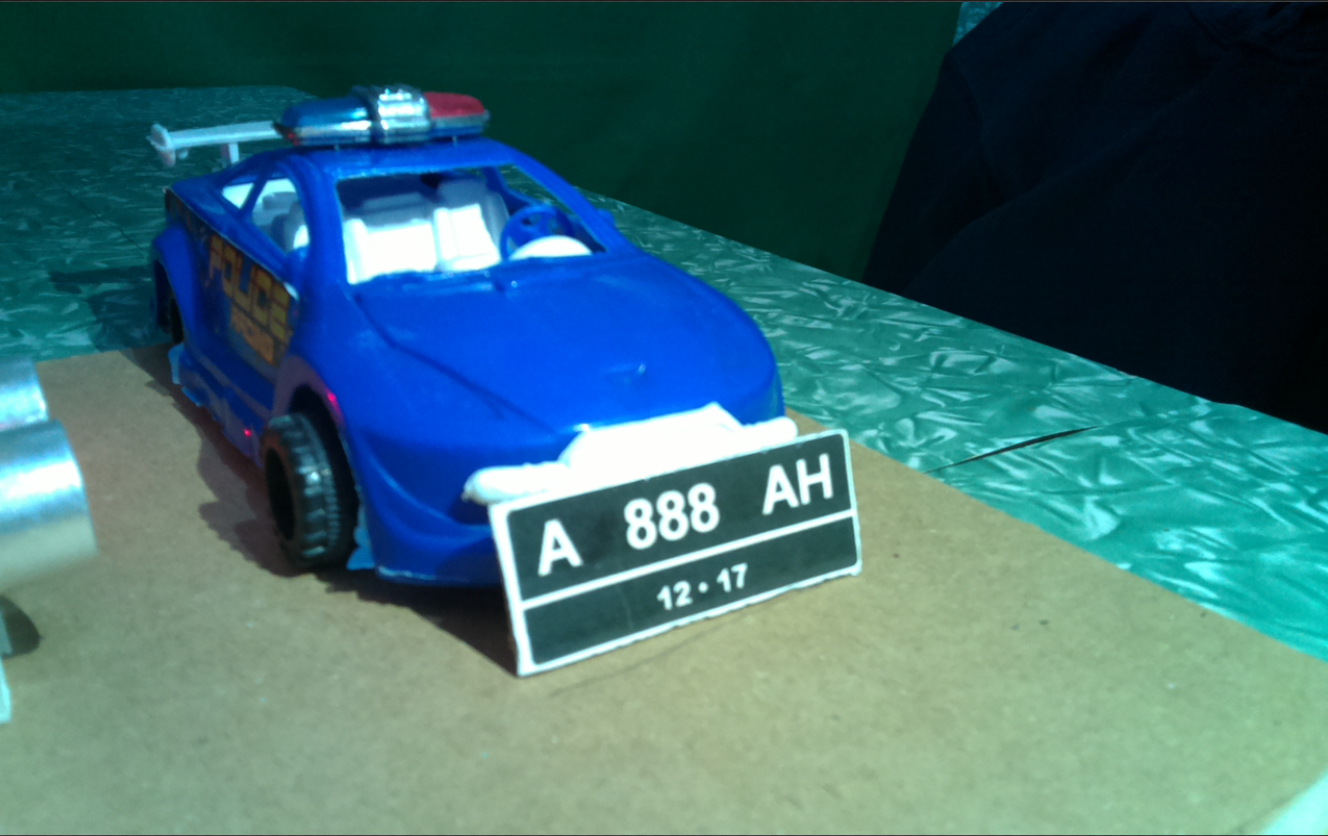
\includegraphics[width=0.85\textwidth, center]{images/Hasil Gambar Kamera Pi.png}
    \caption{Hasil Foto Kamera Pi}
    \label{fig:GambarKameraPi}
\end{figure}

Foto yang diambil oleh kamera akan di proses untuk mengambil nomor plat kendaraan. Pengambilan nomor plat kendaraan menggunakan API(\textit(Aplication Programming Interface)) yang disediakan oleh \textit(platerecognizer.com). Foto yang telah diambil oleh kamera akan dikirim dengan cara mengakses API \textit(platerecognizer.com) yang telah dihubungkan. Setelah berhasil mengakses alamat API, permintaan tersebut akan diteruskan ke server \textit(platerecognizer.com). Jadi, API akan memberitahukan bahwa aplikasi membutuhkan data nomor pelat sesuai gambar yang dikirim. Setelah memproses foto dan menemukan data yang diinginkan, server kembali menghubungi API. Data tersebut berupa nomor plat kendaraan. Selanjutnya, API meneruskan informasi dari server ke aplikasi kita.

% \subsection{Hasil Perancangan Perangkat Lunak}

\section{Hasil Rancangan Aplikasi Web}
Pada penelitian ini menggunakan web sebagai \textit{user interface}. Web yang digunakan dibuat dengan bahasa pemrograman python dan Flask sebagai \textit{framework}nya.

\subsection{\textit{Entity relationship Diagram}}
\begin{figure} [H]
    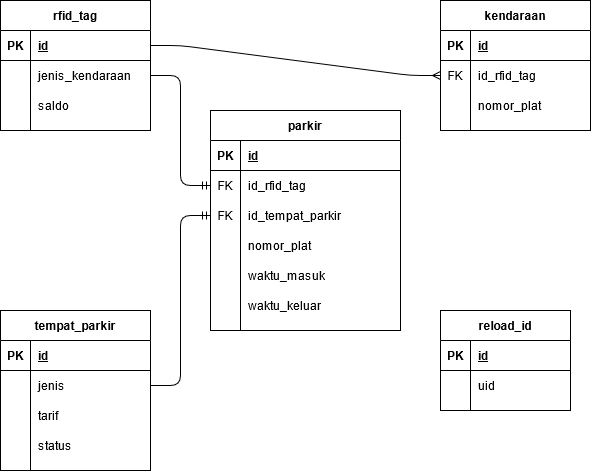
\includegraphics[width=0.85\textwidth, center]{images/er diagram.png}
    \caption{ERD}
    \label{fig:erd}
\end{figure}

Pada gambar ~\ref{fig:erd}, dapat dilihat terdapat 4 tabel yang saling berelasi antar tabel lain dan 1 tabel yang tidak mempunyai relasi antar tabel lain.

\subsection{Struktur \textit{Database}}
Nama \textit{database} : skripsi

Pada \textit{database} aplikasi ini, tabel dibagi menjadi 5 tabel sebagai berikut:

\begin{enumerate}[topsep=0pt,itemsep=0pt,partopsep=0pt, parsep=0pt]
    \item Tabel rfid\_tag

    Nama Tabel : rfid\_tag

    \textit{Primary Key} : id

    \begin{atable}
        \caption{rfid\_tag}
        \label{table:db_rfid_tag}
        \csvreader[
            % column count = 11,
            respect underscore=true,
            tabular=cc,
            head to column names,
            before table=\rowcolors{2}{gray!15}{gray!30},
            table head= \rowcolor{gray!50!black} 
                \color{white} \textit{Coloumn} & 
                \color{white} \textit{Type} 
                \\]
            {tables/db_rfid_tag.csv}
            {
                Coloumn=\Coloumn, 
                Type=\Type}
            {
                \Coloumn & 
                \Type}
    \end{atable}

    Atribut \textit{id} pada tabel rfid\_tag berfungsi sebagai kunci utama. Atribut jenis\_kendaraan digunakan untuk menentukan jenis kendaraan yang digunakan oleh pengemudi. Atribut saldo digunakan untuk menyimpan saldo dari pengemudi.

    \item Tabel tempat\_parkir

    Nama Tabel : tempat\_parkir

    \textit{Primary Key} : id

    \begin{table} [H]
        \centering
        \caption{tempat\_parkir}
        \label{table:db_tempat_parkir}
        \csvreader[
            % column count = 11,
            respect underscore=true,
            tabular=cc,
            head to column names,
            before table=\rowcolors{2}{gray!15}{gray!30},
            table head= \rowcolor{gray!50!black} 
                \color{white} \textit{Coloumn} & 
                \color{white} \textit{Type} 
                \\]
            {tables/db_tempat_parkir.csv}
            {
                Coloumn=\Coloumn, 
                Type=\Type}
            {
                \Coloumn & 
                \Type}
    \end{table}

    Tabel tempat\_parkir mempunyai atribut \textit{id} yang berfungsi sebagai kunci utama, atribut \textit{id} juga berfungsi sebagai nomor slot tempat parkir. Atribut jenis digunakan untuk menentukan jenis dari slot parkir. Atribut tarif digunakan sebagai tarif per jam dari slot parkir. Atribut status digunakan untuk mengetahui apakah slot sedang tersedia atau terpakai.

    \item Tabel kendaraan

    Nama Tabel : kendaraan

    \textit{Primary Key} : id

    \textit{Foreign Key} : id\_rfid\_tag

    \begin{table} [H]
        \centering 
        \caption{kendaraan}
        \label{table:db_kendaraan}
        \csvreader[
            % column count = 11,
            respect underscore=true,
            tabular=cc,
            head to column names,
            respect underscore=true,
            before table=\rowcolors{2}{gray!15}{gray!30},
            table head= \rowcolor{gray!50!black} 
                \color{white} Coloumn & 
                \color{white} Type
                \\]
            {tables/db_kendaraan.csv}
            {
                Coloumn=\Coloumn, 
                Type=\Type}
            {
                \Coloumn & 
                \Type}
    \end{table}

    Tabel kendaraan mempunyai atribut \textit{id} yang berfungsi sebagai kunci utama. Atribut nomor\_plat berfungsi untuk menyimpan nomor plat pengendara. Atribut id\_rfid\_tag didapat dari tabel rfid\_tag.

    \item Tabel parkir

    Nama Tabel : parkir

    \textit{Primary Key} : id

    \textit{Foreign Key} : id\_rfid\_tag, id\_tempat\_parkir

    \begin{table} [H]
        \centering
        \caption{parkir}
        \label{table:db_parkir}
        \csvreader[
            % column count = 11,
            respect underscore=true,
            tabular=cc,
            head to column names,
            before table=\rowcolors{2}{gray!15}{gray!30},
            table head= \rowcolor{gray!50!black} 
                \color{white} \textit{Coloumn} & 
                \color{white} \textit{Type} 
                \\]
            {tables/db_parkir.csv}
            {
                Coloumn=\Coloumn, 
                Type=\Type}
            {
                \Coloumn & 
                \Type}
    \end{table}

    Tabel kendaraan mempunyai atribut \textit{id} yang berfungsi sebagai kunci utama. Atribut id\_rfid\_tag didapat dari tabel rfid\_tag. Atribut nomor\_plat digunakan untuk menyimpan nomor plat pengendara. Atribut id\_tempat\_parkir didapat dari tabel tempat\_parkir. Atribut waktu\_masuk digunakan untuk mencatat waktu masuk pengendara. Atribut waktu\_keluar digunakan untuk mencatat waktu keluar pengguna.

    \item Tabel \textit{reload\_id}

    Nama Tabel : reload\_id

    \textit{Primary Key} : id

    \begin{table} [H]
        \centering
        \caption{reload\_id}
        \label{table:db_reload_id}
        \csvreader[
            % column count = 11,
            respect underscore=true,
            tabular=cc,
            head to column names,
            before table=\rowcolors{2}{gray!15}{gray!30},
            table head= \rowcolor{gray!50!black} 
                \color{white} \textit{Coloumn} & 
                \color{white} \textit{Type} 
                \\]
            {tables/db_reload_id.csv}
            {
                Coloumn=\Coloumn, 
                Type=\Type}
            {
                \Coloumn & 
                \Type}
    \end{table}

    Tabel reload\_id mempunyai atribut \textit{id} yang berfungsi sebagai kunci utama. Atribut uid digunakan untuk menyimpan id rfid tag.

\end{enumerate}

\subsection{Tampilan Website}
Pada tahap ini dilakukan pengimplementasian aplikasi. Berikut penjelasan mengenai tampilan aplikasi.

\subsubsection{Tampilan \textit{Layout} Parkir}
\begin{figure} [H]
    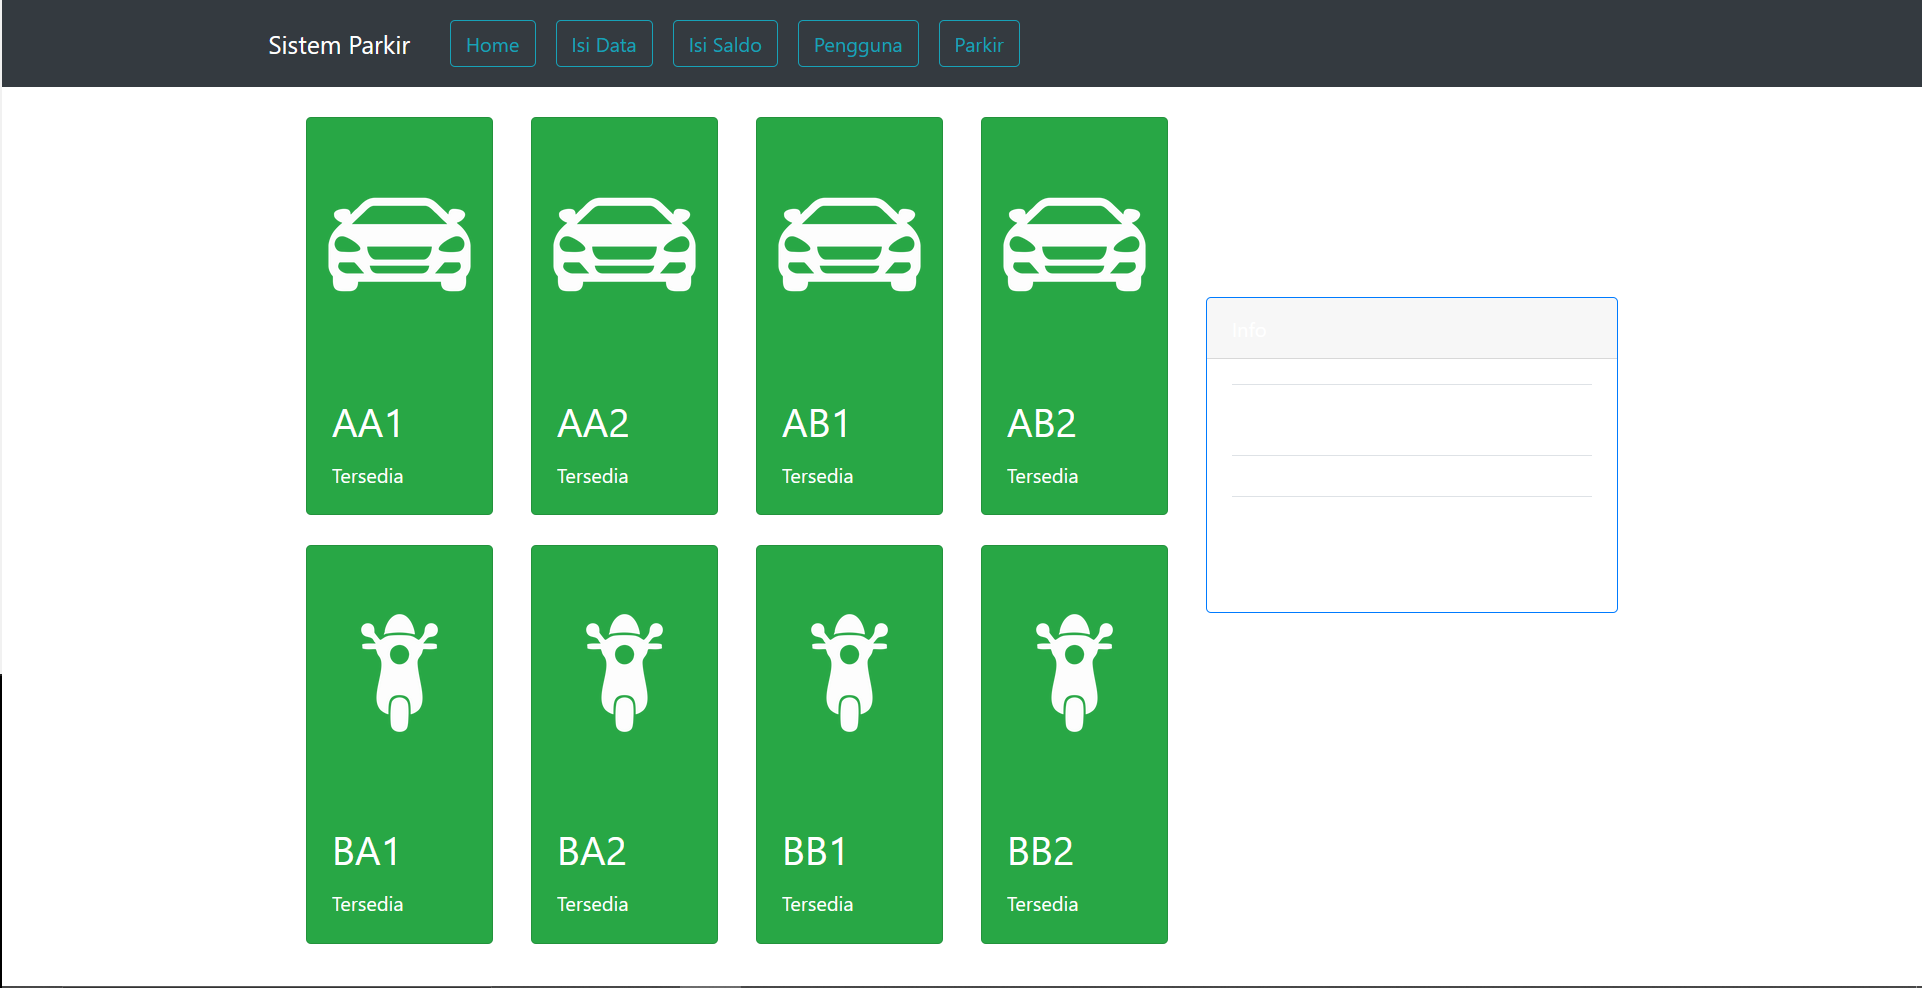
\includegraphics[width=0.85\textwidth, center]{images/web 1 layout parkir.png}
    \caption{\textit{Layout} Parkir}
    \label{fig:web1layout-parkir}
\end{figure}

\textit{Layout} parkir berguna untuk menampilkan informasi mengenai jumlah slot parkir. Pada tampilan kita bisa melihat jumlah slot yang terisi dan terpakai. Pada gambar ~\ref{fig:web1layout-parkir} terlihat jumlah slot parkir ada delapan buah dan semuanya tersedia.\newline

\begin{figure} [H]
    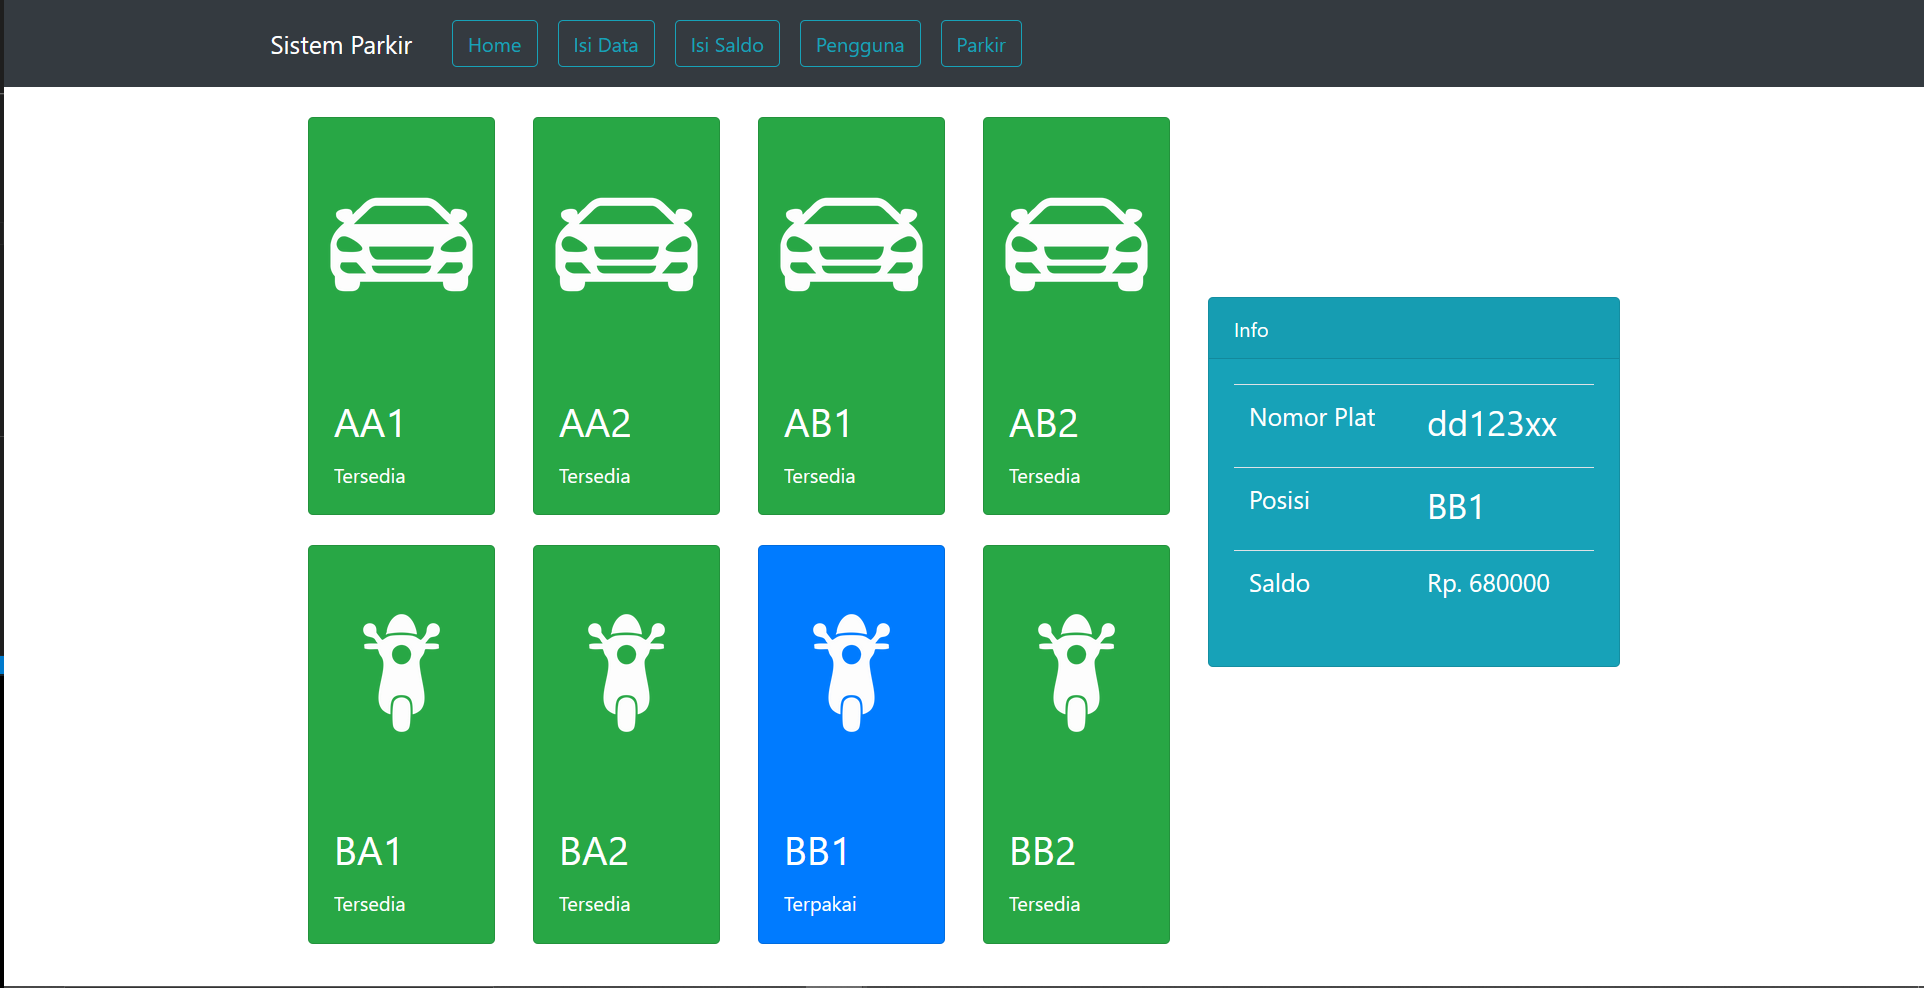
\includegraphics[width=0.85\textwidth, center]{images/web 1 layout parkir baru masuk.png}
    \caption{\textit{Layout} Parkir Saat Pengendara Baru Masuk}
    \label{fig:web1layout-parkir-baru-masuk}
\end{figure}

\begin{figure} [H]
    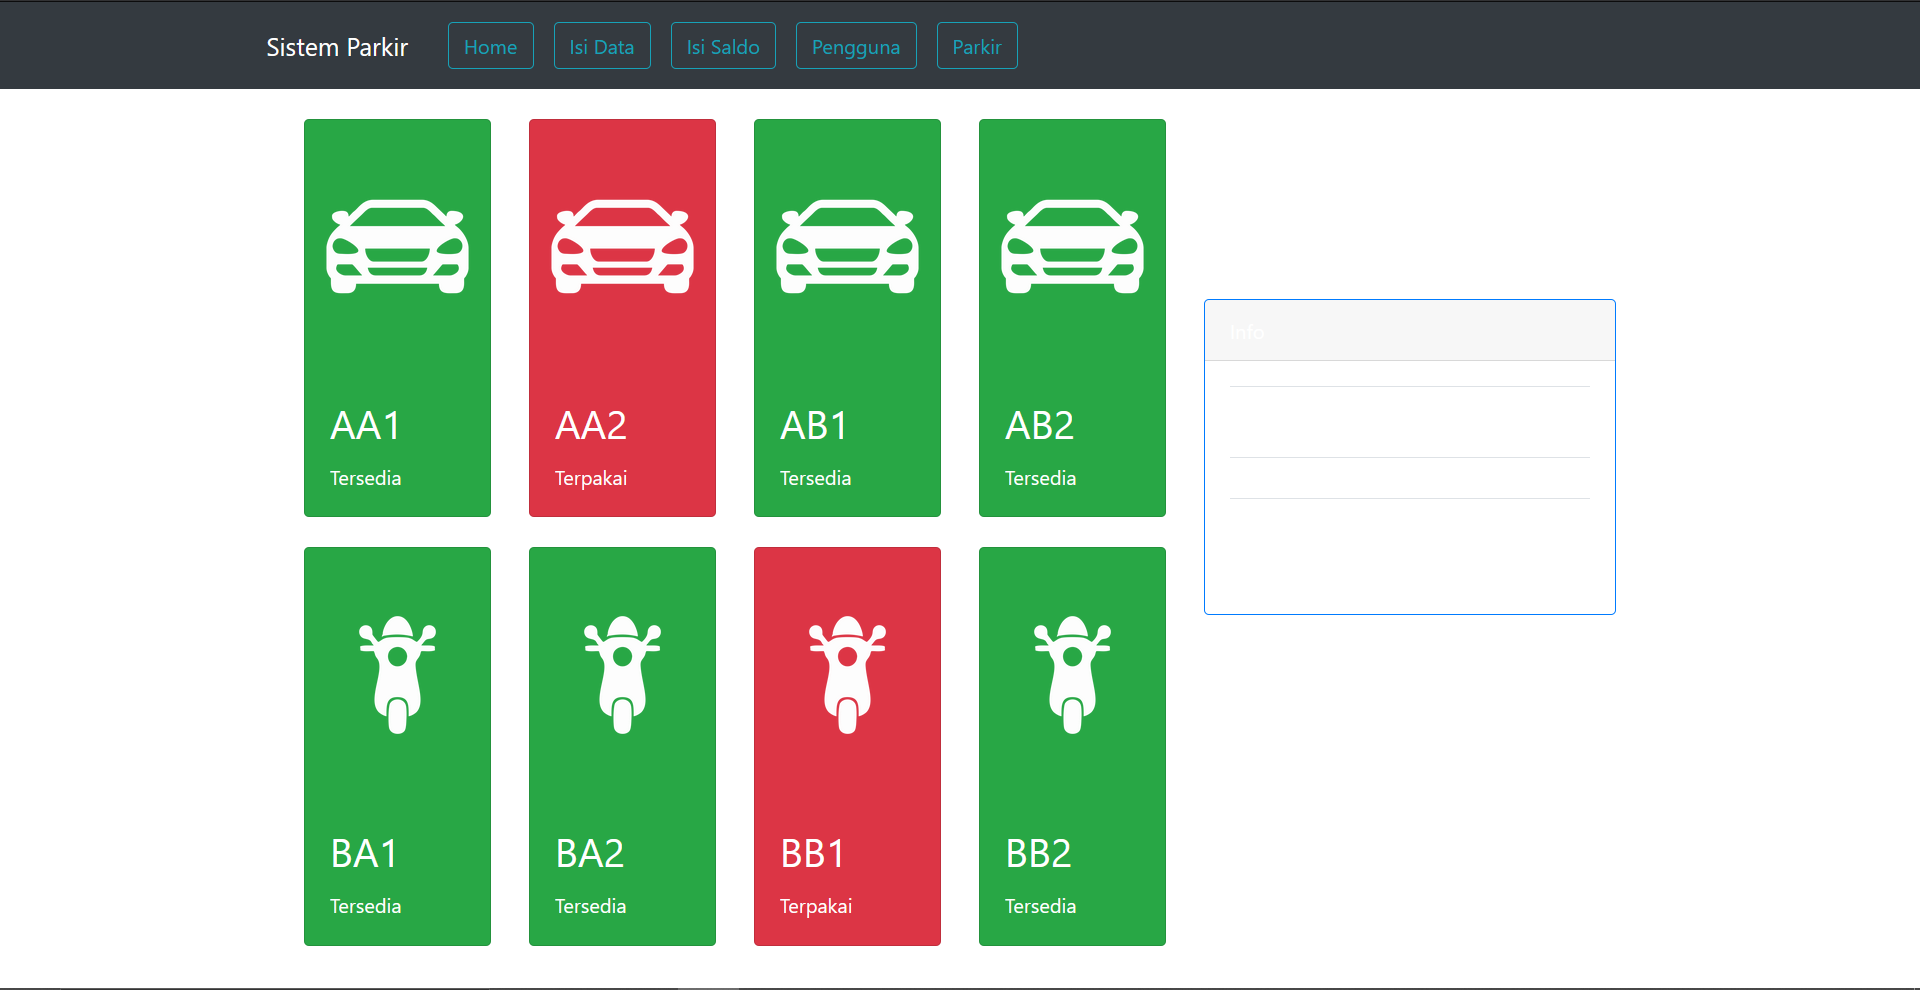
\includegraphics[width=0.85\textwidth, center]{images/web 1 layout parkir ada kendaraan.png}
    \caption{\textit{Layout} Parkir Saat Ada Kendaraan}
    \label{fig:web1layout-parkir-ada-kendaraan}
\end{figure}

Pada gambar ~\ref{fig:web1layout-parkir-baru-masuk} terlihat warna salah satu slot parkir berubah dari warna hijau ke warna biru, ini menunjukan slot yang harus diisi oleh pengendara pada saat baru masuk. Terlihat juga informasi seperti nomor plat, posisi parkir, dan saldo dari pengendara.

Pada gambar ~\ref{fig:web1layout-parkir-ada-kendaraan} terlihat warna slot parkir berubah menjadi warna merah, itu menandakan bahwa slot tersebut sedang terisi.

\subsubsection{Tampilan Isi Data}
\begin{figure} [H]
    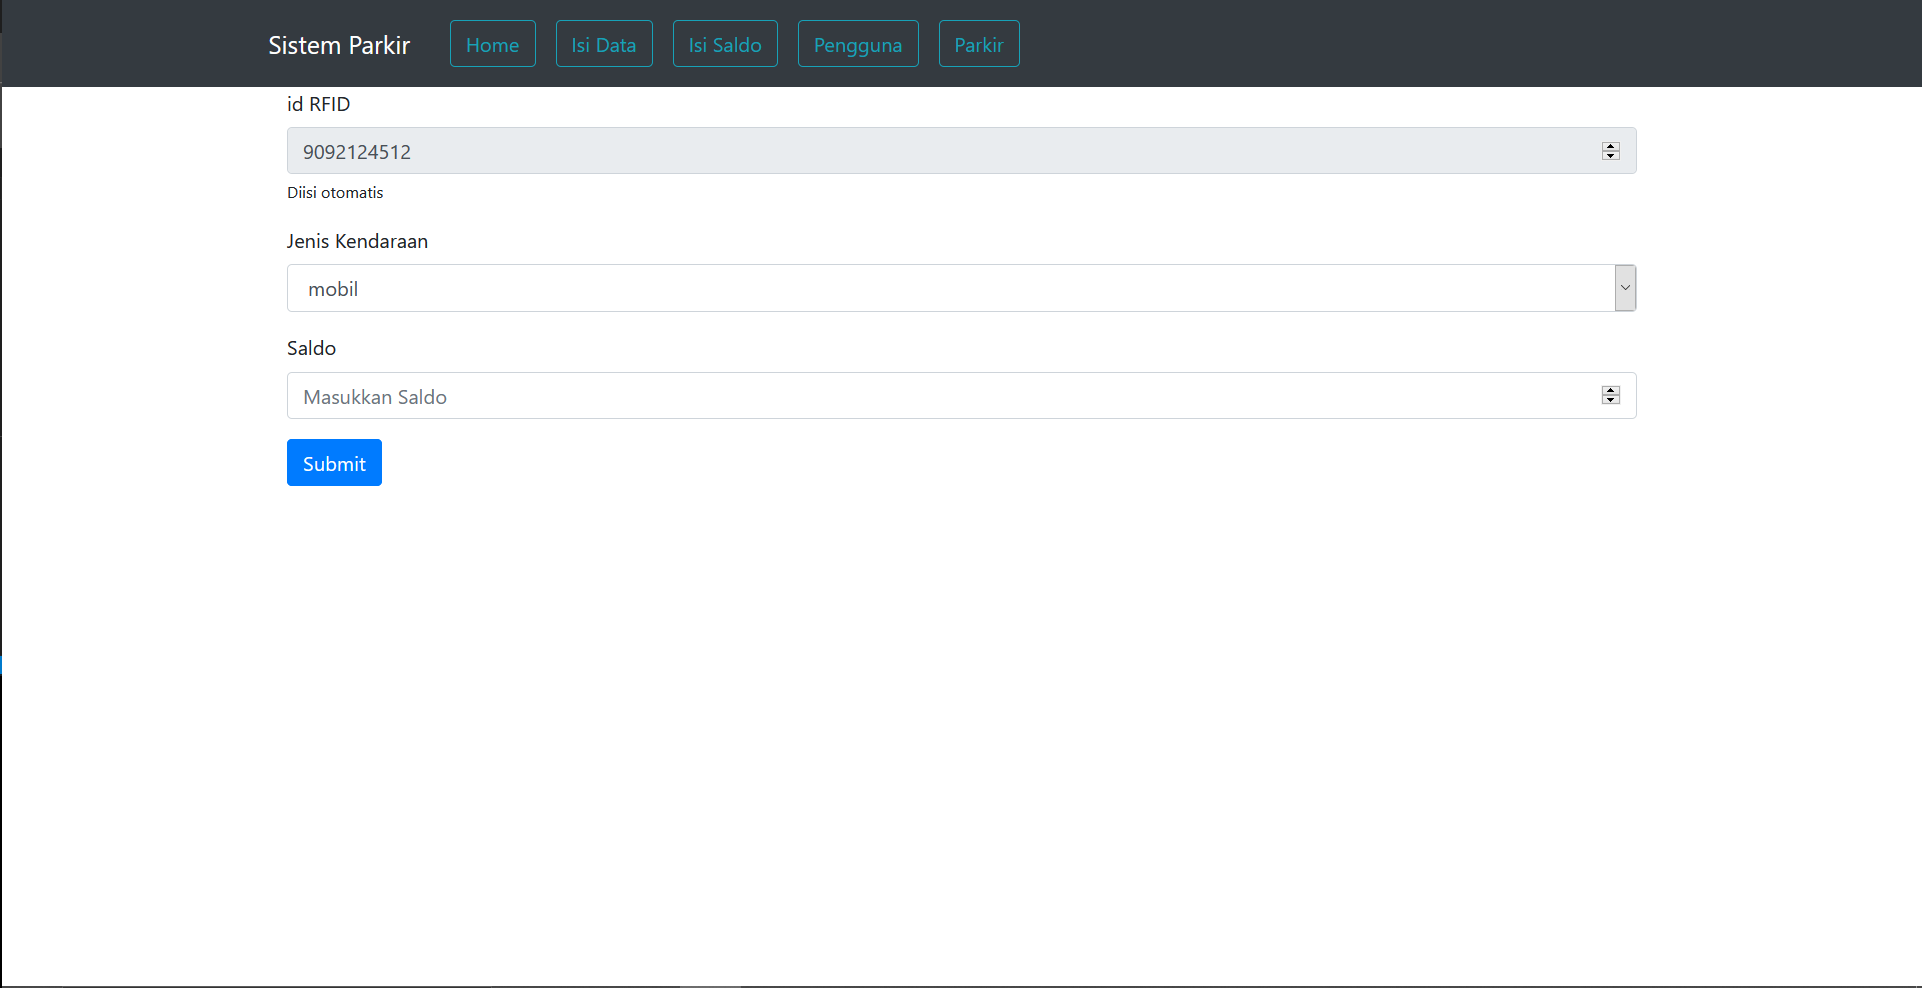
\includegraphics[width=0.85\textwidth, center]{images/web 2 isi data.png}
    \caption{\textit{Form} Isi Data}
    \label{fig:web2isi-data}
\end{figure}

Gambar ~\ref{fig:web2isi-data} merupakan gambar \textit{Form} isi data yang berfungsi untuk memasukkan informasi data pengendara kedalam \textit{database}. Data yang dimasukkan pada \textit{Form} inputan yaitu id RFID, jenis kendaraan, dan saldo. Setelah data diinput maka data akan tersimpan pada \textit{database}.

\subsubsection{Tampilan Isi Saldo}
\begin{figure} [H]
    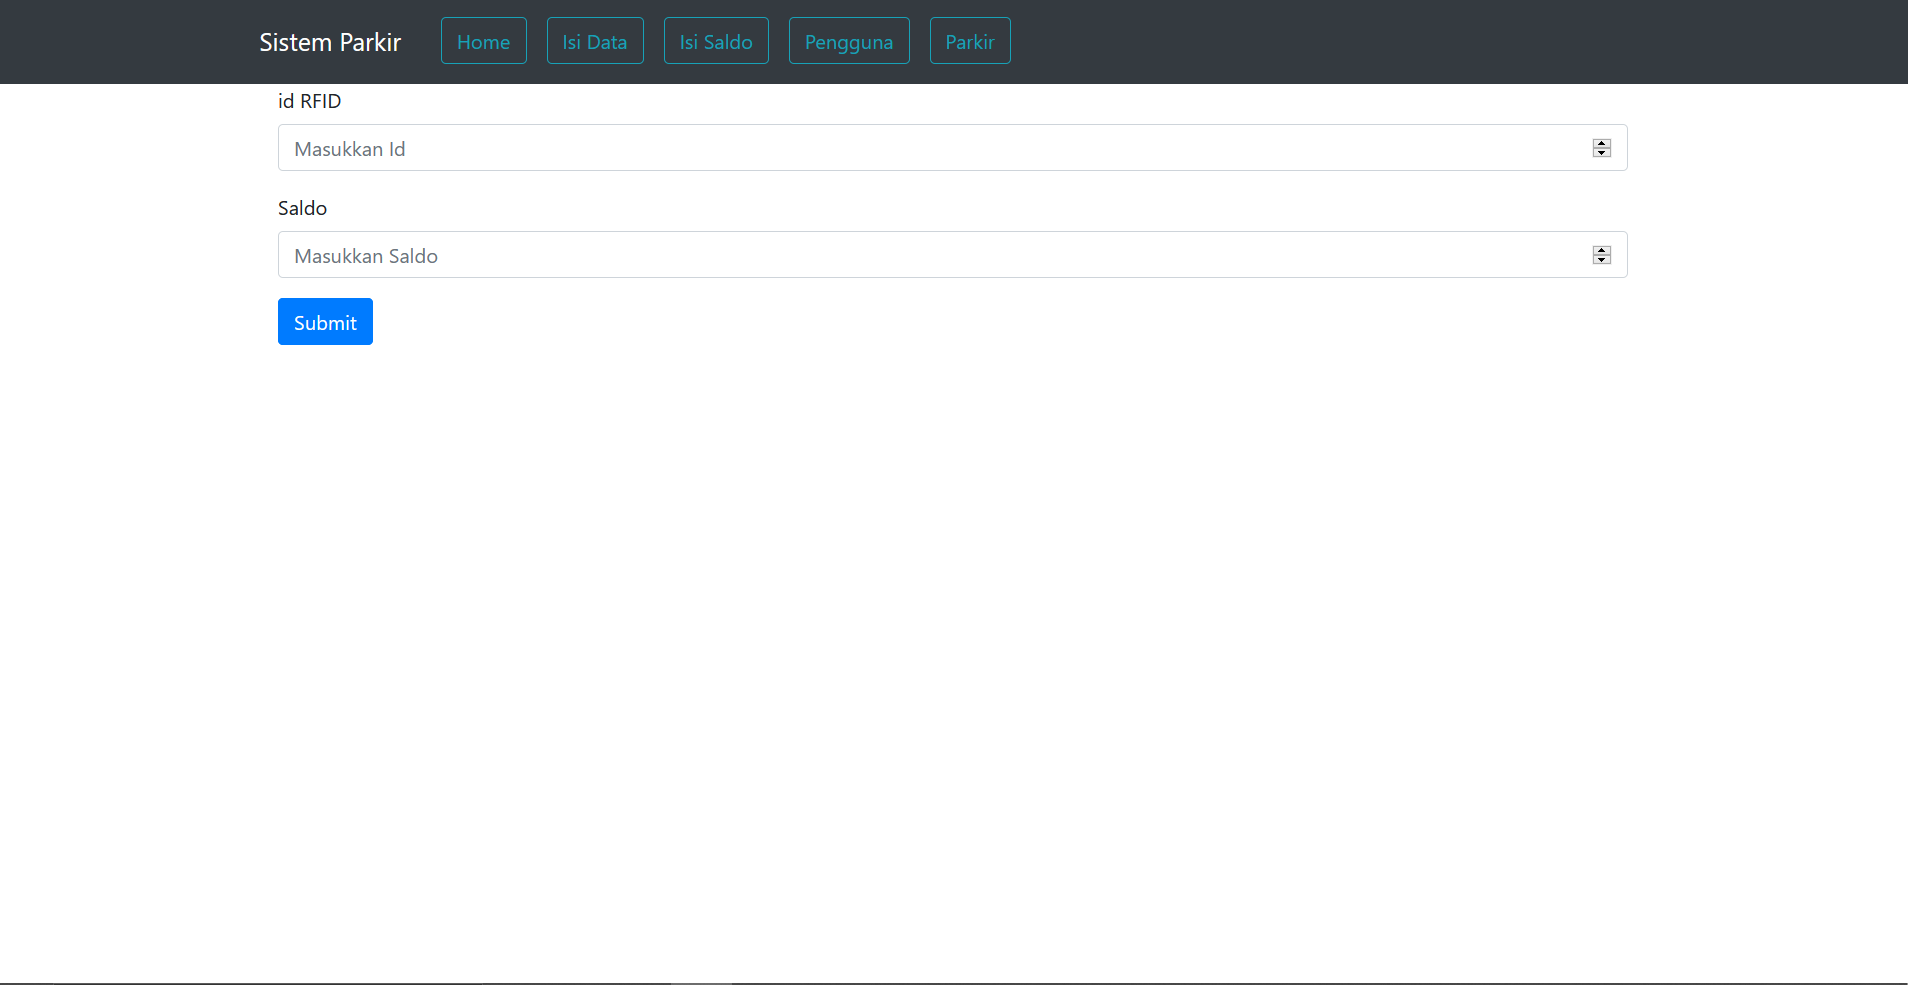
\includegraphics[width=0.85\textwidth, center]{images/web 3 isi saldo.png}
    \caption{\textit{Form} Isi Saldo}
    \label{fig:web3isi-saldo}
\end{figure}

Gambar ~\ref{fig:web3isi-saldo} merupakan gambar \textit{Form} isi saldo yang berfungsi untuk menambahkan saldo pengendara kedalam \textit{database}. Data yang dimasukkan pada \textit{Form} inputan yaitu id RFID dan jumlah saldo yang ingin ditambahkan. Setelah data diinput maka data akan tersimpan pada \textit{database}.

\subsubsection{Tampilan Daftar Pengguna}
\begin{figure} [H]
    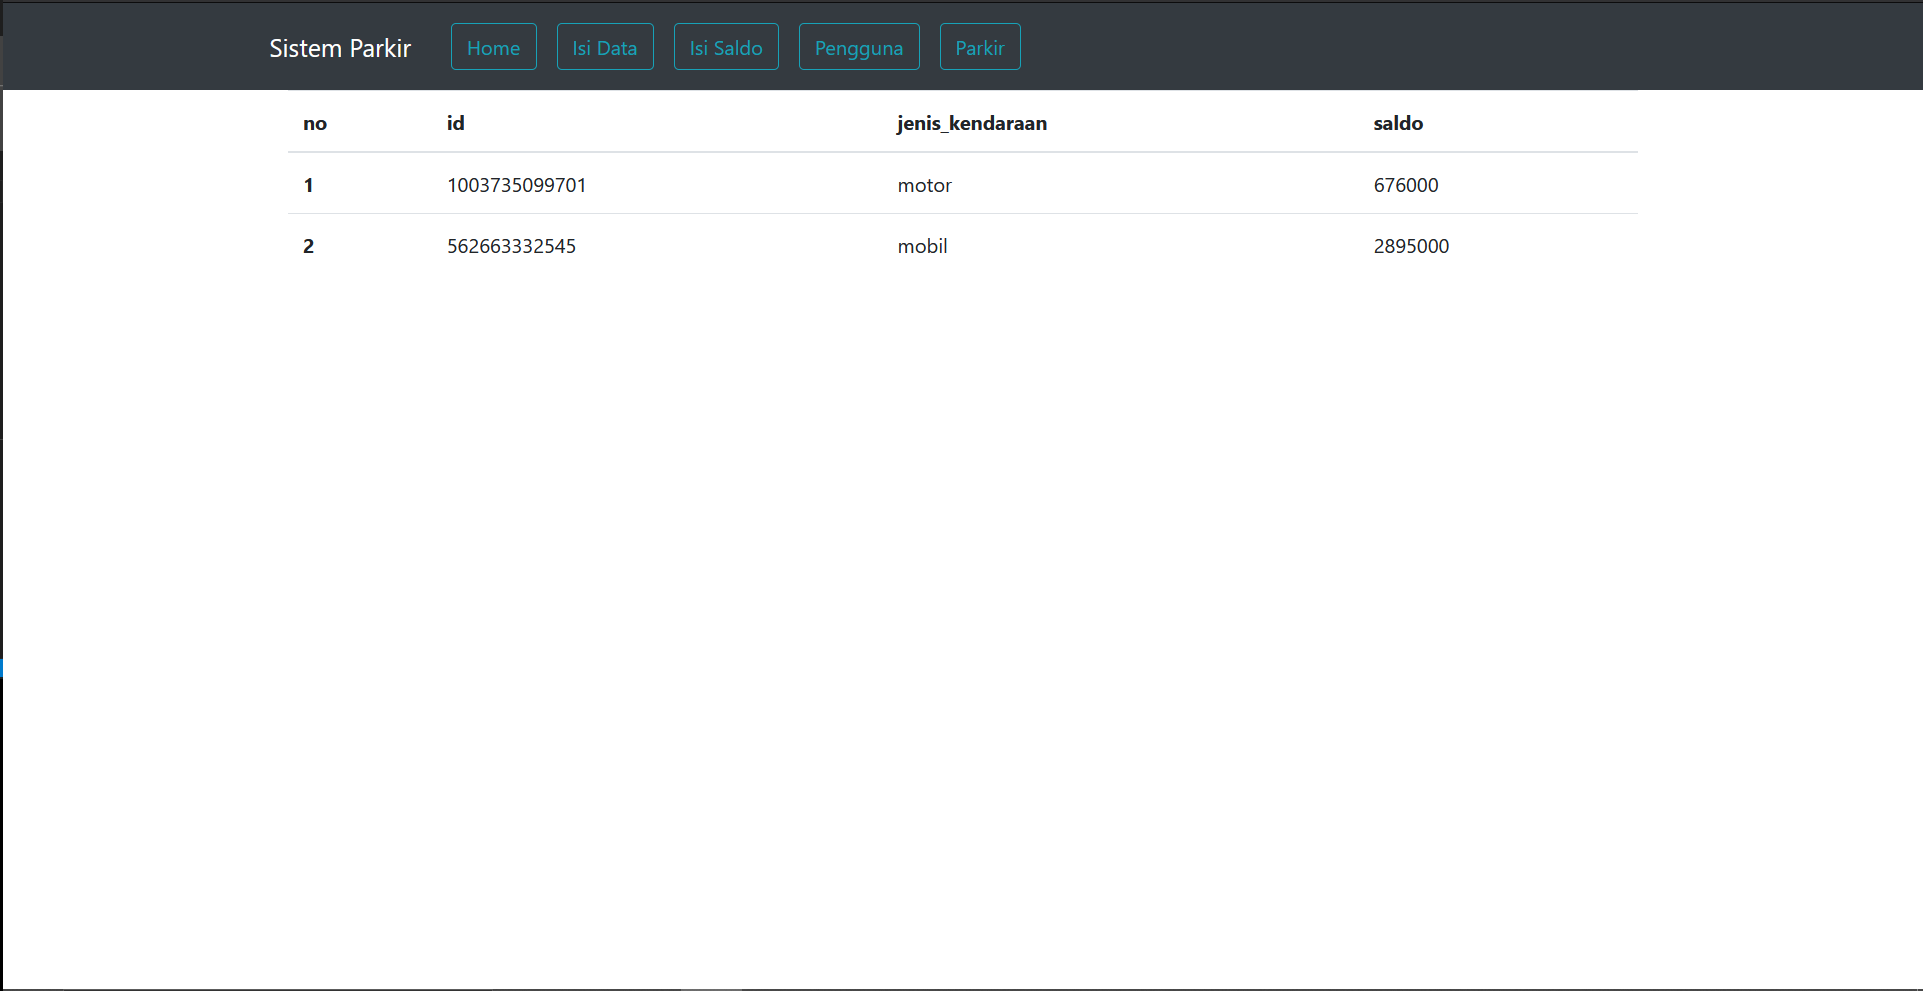
\includegraphics[width=0.85\textwidth, center]{images/web 4 pengguna.png}
    \caption{Daftar Pengguna}
    \label{fig:web4pengguna}
\end{figure}

Gambar ~\ref{fig:web4pengguna} merupakan gambar Tampilan Daftar Pengguna yang berfungsi untuk melihat pengguna yang telah terdaftar. Untuk mendaftarkan pengguna bisa dilakukan di \textit{Form} isi data.

\subsubsection{Tampilan Informasi}
\begin{figure} [H]
    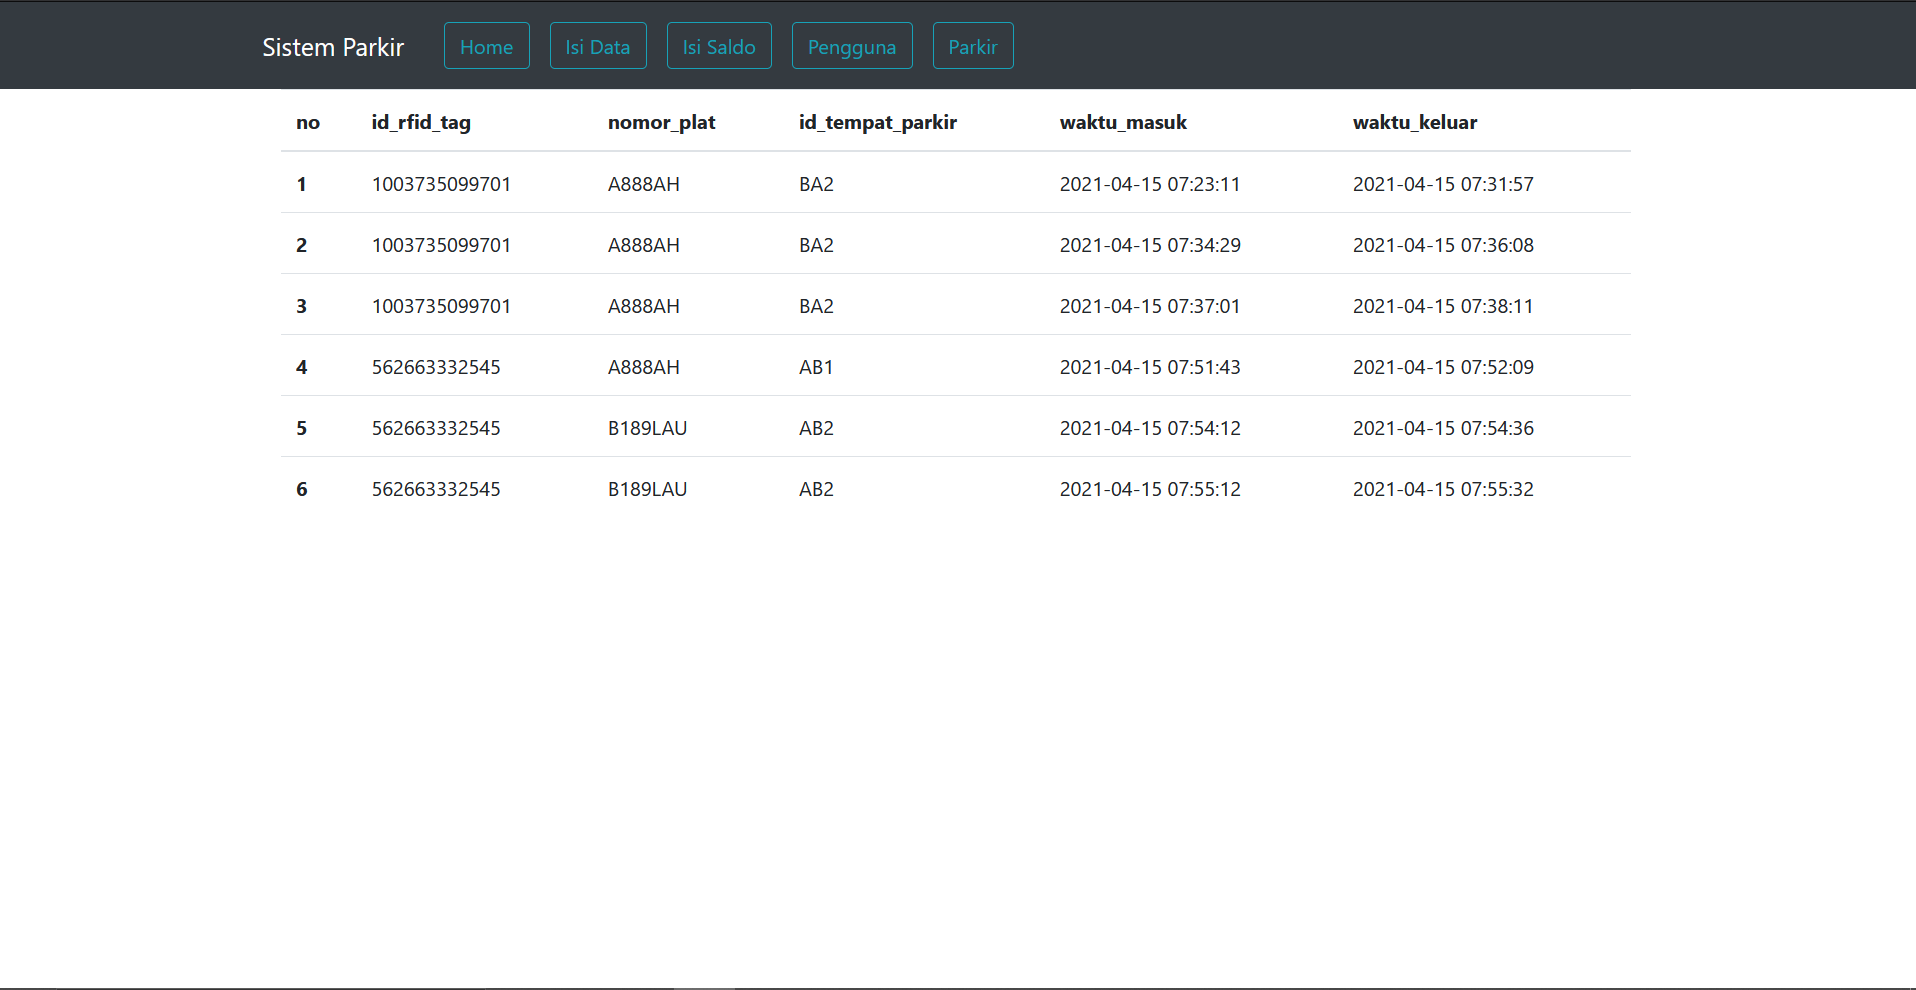
\includegraphics[width=0.85\textwidth, center]{images/web 5 informasi.png}
    \caption{Informasi}
    \label{fig:web5informasi}
\end{figure}

Gambar ~\ref{fig:web5informasi} merupakan gambar Tapilan Informasi yang brrfungsi untuk menampilkan informasi dari pengendara yang sedang parkir. Tampilan ini juga bisa digunakan sebagai tampilan \textit{history} karena manampilkan riwayat parkir semua pengendara.